\documentclass[12pt,a4paper]{report}

% =============================================================================
% PACOTES
% =============================================================================
\usepackage[utf8]{inputenc}
\usepackage[T1]{fontenc}
\usepackage[brazil]{babel}
\usepackage[a4paper,margin=2.5cm]{geometry}
\usepackage{graphicx}
\graphicspath{{figures/}}
\usepackage{booktabs}
\usepackage{longtable}
\usepackage{amsmath}
\usepackage{amssymb}
\usepackage{xcolor}
\usepackage{caption}
\usepackage{subcaption}
\usepackage{float}
\usepackage{array}
\usepackage{enumitem}
\usepackage{setspace}
\usepackage{titlesec}
\usepackage[colorlinks=true,linkcolor=blue!50!black,citecolor=blue!50!black,urlcolor=blue!50!black]{hyperref}

\onehalfspacing
\captionsetup{font=small,labelfont=bf,margin=1cm}
\titleformat{\chapter}[hang]{\normalfont\huge\bfseries}{\thechapter.}{20pt}{\huge}

% =============================================================================
% DADOS DO DOCUMENTO
% =============================================================================
\title{\textbf{Abordagem Espectral com Assinaturas Harmônicas e\\
Interharmônicas para Desagregação de Cargas e\\
Manutenção Preditiva em Sistemas Trifásicos}\\[0.4cm]
\large Relatório Consolidado de Metodologia, Construção do Sistema e Resultados}
\author{Relatório de progresso de pesquisa de doutorado}
\date{\today}

\begin{document}

\maketitle

% =============================================================================
% RESUMO
% =============================================================================
\begin{abstract}
\noindent
Este trabalho apresenta uma metodologia de análise espectral que utiliza
diretamente componentes harmônicas e interharmônicas, fornecidas por
analisadores de energia, para realizar simultaneamente a detecção de falhas
iminentes e a desagregação de cargas em sistemas trifásicos. Os dados são
obtidos em bancadas experimentais com retificador trifásico alimentando carga
em corrente contínua e um conjunto moto-máquina ajustável submetido a
desequilíbrios de massa e desalinhamentos (defeitos em rolamentos estão
previstos no desenho experimental, mas ainda não integram a base de dados
analisada nesta etapa — Capítulo~\ref{ch:limitacoes}). O banco de dados
contempla condições normais de operação, falhas isoladas — elétricas ou
mecânicas — e falhas combinadas, de modo a registrar assinaturas espectrais
representativas de cada cenário. As amplitudes das componentes espectrais nas
três fases constituem vetores de características que alimentam dois modelos
dedicados: um classificador com rede neural recorrente para o diagnóstico de
modos de falha (17 condições — saudável, elétrica, mecânica e combinada) e um
modelo de regressão multi-saída para a desagregação de cargas em operação
simultânea. Um pipeline computacional reprodutível de 13 módulos foi
construído para importar, validar, organizar, normalizar, analisar
estatisticamente e modelar uma base de dados experimental com 19.501
aquisições e 17 condições. Os resultados confirmam a viabilidade de um
sistema não invasivo, capaz de identificar cargas ativas (evidência real,
porém parcial, de desagregação — R\textsuperscript{2} até 0,214 por canal,
tratada como estudo de viabilidade dado o número reduzido de condições
combinadas disponíveis) e de diagnosticar precocemente falhas elétricas,
mecânicas e combinadas (acurácia estável de 91--92\% sob validação cruzada
nas 17 condições), fortalecendo estratégias de manutenção preditiva em
ambientes industriais. Uma sub-análise de apoio, restrita às condições
mecânicas isoladas de qualquer influência elétrica, identifica quais
componentes espectrais especificamente carregam sinal mecânico
($\eta^2$ até 0,95), reforçando a interpretabilidade do diagnóstico geral.
Este relatório reúne todas as figuras produzidas ao longo da pesquisa — desde
a exploração inicial da base de dados até a validação cruzada dos
classificadores e a separabilidade visual das classes — acompanhadas de
metodologia, interpretação, limitações e proposta de trabalhos futuros.
\end{abstract}

\tableofcontents
\listoffigures
\listoftables

% =============================================================================
% LISTA DE ABREVIATURAS E SIGLAS
% =============================================================================
\chapter*{Lista de Abreviaturas e Siglas}
\addcontentsline{toc}{chapter}{Lista de Abreviaturas e Siglas}

\begin{description}[style=multiline,leftmargin=3.2cm,font=\normalfont\bfseries\ttfamily]
\item[ANOVA] \emph{Analysis of Variance} — análise de variância (teste estatístico multi-grupo)
\item[BiLSTM] \emph{Bidirectional Long Short-Term Memory} — LSTM bidirecional
\item[CNN] \emph{Convolutional Neural Network} — rede neural convolucional
\item[CV] \emph{Cross-Validation} — validação cruzada
\item[DC] \emph{Direct Current} — componente de corrente/tensão contínua (ordem 0)
\item[FDR] \emph{False Discovery Rate} — taxa de descoberta falsa (correção de Benjamini-Hochberg)
\item[GRU] \emph{Gated Recurrent Unit} — unidade recorrente com portões
\item[H] Harmônica (ordem inteira da frequência fundamental)
\item[IH] Inter-harmônica (componente espectral entre ordens harmônicas inteiras)
\item[k-NN] \emph{k-Nearest Neighbors} — k vizinhos mais próximos
\item[LogReg] Regressão Logística
\item[LSTM] \emph{Long Short-Term Memory} — memória de longo-curto prazo
\item[MAE] \emph{Mean Absolute Error} — erro absoluto médio
\item[MCSA] \emph{Motor Current Signature Analysis} — análise de assinatura de corrente do motor
\item[MHA] \emph{Multi-Head Attention} — atenção multi-cabeça (mecanismo do Transformer)
\item[MLP] \emph{Multi-Layer Perceptron} — perceptron multicamadas
\item[MSE] \emph{Mean Squared Error} — erro quadrático médio
\item[NILM] \emph{Non-Intrusive Load Monitoring} — monitoramento não intrusivo de cargas (desagregação)
\item[PC1, PC2] Primeira e segunda componentes principais
\item[PCA] \emph{Principal Component Analysis} — análise de componentes principais
\item[RF] \emph{Random Forest} — floresta aleatória
\item[RNN] \emph{Recurrent Neural Network} — rede neural recorrente
\item[RQ1] \emph{Research Question} 1 — diagnóstico de modos de falha (17 condições) para manutenção preditiva
\item[RQ2] \emph{Research Question} 2 — desagregação de cargas (NILM)
\item[RUL] \emph{Remaining Useful Life} — vida útil remanescente (tempo até a falha)
\item[SHAP] \emph{SHapley Additive exPlanations} — método de interpretabilidade baseado em valores de Shapley
\item[SVM] \emph{Support Vector Machine} — máquina de vetores de suporte
\item[TID-F] Taxa de distorção inter-harmônica relativa à fundamental
\item[THD] \emph{Total Harmonic Distortion} — distorção harmônica total
\item[THDe, THDo] THD das harmônicas pares (\emph{even}) e ímpares (\emph{odd})
\item[THD3] THD das harmônicas múltiplas de 3 (triplens)
\item[XGBoost] \emph{Extreme Gradient Boosting}
\end{description}

% =============================================================================
% LISTA DE SÍMBOLOS
% =============================================================================
\chapter*{Lista de Símbolos}
\addcontentsline{toc}{chapter}{Lista de Símbolos}

\begin{description}[style=multiline,leftmargin=3.2cm,font=\normalfont\bfseries]
\item[$\eta^2$] Eta ao quadrado — tamanho de efeito multi-grupo (proporção da variância total explicada pela condição); usado para dimensionar o resultado de um teste ANOVA
\item[$\delta$] Delta de Cliff — tamanho de efeito não-paramétrico par-a-par, no intervalo $[-1, 1]$
\item[$p$] Valor-\emph{p} — probabilidade de observar o efeito medido (ou maior) sob a hipótese nula
\item[$p_{\text{adj}}$] Valor-\emph{p} ajustado pela correção de Benjamini-Hochberg (FDR)
\item[$\alpha$] Nível de significância adotado (0,05 neste trabalho)
\item[$R^2$] Coeficiente de determinação (proporção da variância do alvo explicada pelas previsões)
\item[$H_n$] $n$-ésima ordem harmônica (ex.: $H_5$ = quinta harmônica)
\item[$IH_n$] $n$-ésima ordem inter-harmônica
\item[$V_a, V_b, V_c$] Tensão de fase A, B e C
\item[$I_a, I_b, I_c$] Corrente de fase A, B e C
\item[$|\phi|$] Valor absoluto médio de Shapley (importância SHAP)
\end{description}

% =============================================================================
% CAPÍTULO 1 — INTRODUÇÃO
% =============================================================================
\chapter{Introdução}

Sistemas elétricos trifásicos com cargas não-lineares (retificadores) e
máquinas rotativas produzem, além da componente fundamental de 60~Hz, um
espectro de harmônicas e inter-harmônicas de tensão e corrente. A hipótese de
trabalho desta pesquisa é que esse espectro carrega informação diagnóstica
tanto sobre o estado mecânico da máquina (desbalanceamento, desalinhamento)
quanto sobre a composição das cargas elétricas conectadas ao sistema —
informação que, em princípio, poderia ser extraída sem instrumentação
adicional além do próprio analisador de energia já presente em instalações
industriais. O objetivo central não é estudar essas duas fontes de
informação isoladamente, mas construir, a partir do mesmo tipo de dado de
entrada (assinatura espectral agregada, sem forma de onda bruta), um sistema
único capaz de (a) diagnosticar precocemente o modo de falha do sistema —
elétrico, mecânico ou combinado — para suportar manutenção preditiva, e (b)
desagregar a contribuição espectral de cargas elétricas operando
simultaneamente no mesmo ponto de acoplamento comum.

\section{Perguntas de pesquisa}

Duas perguntas, tratadas como objetivos co-primários, orientam a
investigação:

\begin{itemize}
\item \textbf{RQ1 (diagnóstico e manutenção preditiva)} — Um modelo treinado
sobre a assinatura espectral consegue diagnosticar corretamente o modo de
falha do sistema — saudável, falha elétrica isolada, falha mecânica isolada
ou falha combinada, 17 condições ao todo — com desempenho suficiente para
suportar detecção precoce de falha?
\item \textbf{RQ2 (desagregação de cargas / NILM)} — Com duas cargas
elétricas operando simultaneamente no mesmo ponto de acoplamento comum, é
possível desagregá-las usando exclusivamente a assinatura espectral, sem
recorrer à forma de onda bruta?
\end{itemize}

\noindent Como evidência de apoio à interpretabilidade de RQ1 — não como uma
terceira pergunta independente — este relatório inclui também uma
\textbf{sub-análise de sensibilidade mecânica isolada}: restringindo o
universo de análise às condições mecânicas puras (sem nenhuma falha elétrica
presente), quais componentes espectrais especificamente carregam sinal
mecânico genuíno, e com que tamanho de efeito? Isolar a variável mecânica do
efeito de confusão elétrico (qualquer harmônico de corrente é, por
construção, sensível à presença de uma carga não-linear) fortalece a
interpretação do diagnóstico geral sobre as classes mecânicas.

\noindent As hipóteses correspondentes são: (H-RQ1) um classificador
supervisionado (rede neural recorrente como modelo principal, modelos
clássicos como baseline) atinge acurácia e F1-macro substancialmente acima do
acaso nas 17 condições, incluindo discriminação entre falha elétrica,
mecânica e combinada; (H-RQ2) um modelo supervisionado treinado sobre a
assinatura combinada consegue recuperar a assinatura da fonte elétrica
individual com desempenho consistentemente acima de um preditor trivial,
avaliado em condições combinadas nunca vistas no treino; (H-sensibilidade)
pelo menos um subconjunto de ordens harmônicas/inter-harmônicas de corrente
ou tensão apresenta separação estatisticamente significativa (ANOVA com
correção FDR) e com tamanho de efeito não desprezível ($\eta^2 \geq 0{,}06$)
entre as condições mecânicas puras.

\section{Nota de aderência entre o desenho experimental e este relatório}

Três esclarecimentos evitam ambiguidade de leitura deste documento frente ao
desenho experimental real: (1) o rótulo \texttt{RET~N~PARAF} (Seção~
\ref{sec:taxonomia}) é literalmente a quantidade de parafusos retirados de um
disco calibrado da bancada moto-máquina para induzir desbalanceamento —
confirmado diretamente com o pesquisador responsável pelo ensaio, não apenas
inferido por similaridade espectral; (2) defeitos em rolamentos fazem parte
do desenho experimental da bancada, mas ainda não estão presentes no banco de
dados analisado nesta etapa (Capítulo~\ref{ch:limitacoes}); (3) a
desagregação de cargas (RQ2) é implementada com um modelo de regressão
multi-saída baseado em \emph{Random Forest}, não com uma rede neural
recorrente — o dataset de condições combinadas ($n=4$) é pequeno demais para
justificar a complexidade adicional de uma arquitetura recorrente frente a
uma alternativa mais simples e igualmente válida (Seção~2.4).

\section{Estrutura do documento}

O Capítulo~2 descreve a metodologia (base de dados, taxonomia experimental,
protocolo estatístico, modelos de aprendizado de máquina e redes neurais,
métricas). O Capítulo~3 descreve a arquitetura do sistema computacional
construído para executar essa metodologia de forma reprodutível. O
Capítulo~4 apresenta a totalidade dos resultados obtidos, organizados
cronologicamente pela ordem em que foram produzidos ao longo da pesquisa —
da exploração inicial da base de dados até a validação cruzada final dos
classificadores — com uma figura (ou grupo de figuras) por achado e a
interpretação correspondente; a Seção~\ref{sec:full-pipeline} concentra a
evidência primária de RQ1 (diagnóstico nas 17 condições) e a
Seção~\ref{sec:nilm-ressalva} a evidência primária de RQ2 (NILM), com a
sub-análise de sensibilidade mecânica isolada posicionada como apoio
interpretativo (Seção~\ref{sec:etapa1}). O Capítulo~5 discute os resultados à
luz das perguntas de pesquisa; o Capítulo~6 lista as limitações
identificadas; o Capítulo~7 propõe trabalhos futuros; o Capítulo~8 conclui o
documento.

% =============================================================================
% CAPÍTULO 2 — METODOLOGIA
% =============================================================================
\chapter{Metodologia}

\section{Base de dados}

A base de dados experimental (\texttt{BANCO\_DADOS\_CONSOLIDADO.xlsx}) é
composta por duas planilhas — \textsc{Harmônicas} (672 colunas) e
\textsc{Interharmônicas} (626 colunas) — cada uma com 19.501 aquisições,
cobrindo 17 condições experimentais de um motor de indução trifásico. Cada
planilha registra harmônicas ou inter-harmônicas de ordem 1 a 50 (estatísticas
média e máxima), para tensão e corrente, nas três fases, além das famílias
THD, THDo, THDe, THD3, K-Factor e TID-F. As duas planilhas constituem séries
temporais independentes do mesmo ensaio — os instantes de aquisição
(\texttt{Registro}) não coincidem entre elas — e são pareadas por rótulo e
proximidade temporal quando uma análise exige as duas simultaneamente
(\emph{nearest-timestamp join}, tolerância de 90~s).

Durante a validação da base de dados foi identificado que as colunas
\texttt{H00}--\texttt{H50~max} aparecem com nome idêntico nas duas planilhas.
A comparação par-a-par dos valores (pareados por rótulo e timestamp mais
próximo) revelou 85,81\% de divergência entre eles (306 canais comparados,
5.967.306 pares, diferença absoluta máxima de 136,97 pontos percentuais) —
não são duplicatas, mas fontes de dado distintas, mantidas como atributos
separados no conjunto combinado (Seção~\ref{sec:validacao}, Figura~\ref{fig:findings-hmax}).

\section{Taxonomia experimental}
\label{sec:taxonomia}

Os 17 rótulos experimentais foram particionados em três categorias
mutuamente exclusivas — todas as 17 compõem o problema de diagnóstico geral
(RQ1); o subconjunto mecânico puro é reaproveitado à parte para a
sub-análise de sensibilidade isolada (Tabela~\ref{tab:taxonomia}):

\begin{table}[H]
\centering
\caption{Taxonomia experimental dos 17 rótulos da base de dados.}
\label{tab:taxonomia}
\begin{tabular}{@{}lrrl@{}}
\toprule
\textbf{Categoria} & \textbf{N.\ rótulos} & \textbf{N.\ amostras} & \textbf{Papel na pesquisa} \\
\midrule
Mecânica pura & 6 & 8.814 & RQ1 (diagnóstico) + sub-análise de sensibilidade isolada \\
Elétrica pura & 7 & 4.580 & RQ1 (diagnóstico) + fonte elétrica de referência para RQ2 \\
Combinada (máquina + elétrica) & 4 & 6.107 & RQ1 (diagnóstico) + RQ2 — desagregação supervisionada \\
\midrule
\textbf{Total} & \textbf{17} & \textbf{19.501} & --- \\
\bottomrule
\end{tabular}
\end{table}

\noindent Os experimentos têm duas origens físicas independentes, monitoradas
pelo mesmo conjunto de analisadores de energia: um retificador trifásico
alimentando carga em corrente contínua, do qual diodos foram progressivamente
removidos para induzir falha elétrica (\texttt{DIODO~1}--\texttt{6},
\texttt{RETIFICADOR COMPLETO}); e uma bancada moto-máquina ajustável, na qual
desbalanceamento é induzido retirando parafusos de um disco calibrado e
desalinhamento é ajustado mecanicamente. O sufixo \texttt{RET~N~PARAF} é
literalmente a quantidade de parafusos retirados do disco para cada grau de
desbalanceamento (\texttt{RET~15~PARAF} combina isso com desalinhamento) —
confirmado diretamente com o pesquisador responsável pelo ensaio, consistente
com a observação empírica de que o perfil harmônico de corrente desses
rótulos é estatisticamente indistinguível do perfil da condição saudável, e
discrepante do perfil das condições com retificador conectado.

\section{Protocolo de diagnóstico e manutenção preditiva (RQ1)}
\label{sec:protocolo-diagnostico}

Universo de análise: as 17 condições experimentais completas (Tabela~
\ref{tab:taxonomia}), todas as famílias espectrais disponíveis. O modelo
principal é uma rede neural recorrente treinada sobre janelas de aquisições
consecutivas (seis arquiteturas comparadas — Seção~2.4); modelos clássicos
(Random Forest, XGBoost, SVM, MLP, k-NN, Regressão Logística) servem de
baseline sem contexto temporal. Avaliação por validação cruzada estratificada
de 5 dobras, acurácia e F1-macro, agregados e por classe. Interpretabilidade
via SHAP e \emph{permutation importance} sobre o modelo clássico de melhor
desempenho.

\section{Sub-análise de sensibilidade mecânica isolada (apoio interpretativo a RQ1)}
\label{sec:protocolo-estatistico}

Como controle metodológico que isola a variável mecânica do efeito de
confusão elétrico — não como um objetivo autônomo da tese — para cada canal
espectral (domínio $\times$ família $\times$ variável $\times$ fase $\times$
ordem $\times$ estatística), aplicou-se ANOVA de um fator entre as 6
condições mecânicas puras, seguida de correção de Benjamini-Hochberg (FDR,
$\alpha=0{,}05$) sobre o conjunto completo de canais testados
simultaneamente. Como tamanho de efeito multi-grupo, calculou-se $\eta^2$
(proporção de variância explicada pela condição); para contrastes par-a-par
(cada falha mecânica \emph{vs.} baseline saudável), utilizou-se o delta de
Cliff não-paramétrico. Um classificador multi-classe restrito às condições
mecânicas, com importância de atributos via SHAP e \emph{permutation
importance}, serviu de validação cruzada independente do ranking estatístico
— a concordância entre os dois métodos (estatístico e baseado em modelo)
fortalece a evidência sobre quais canais carregam sinal mecânico genuíno,
reforçando a interpretação das mesmas classes dentro do diagnóstico geral
(Seção~\ref{sec:protocolo-diagnostico}).

\section{Modelos de aprendizado de máquina e redes neurais}

Seis modelos clássicos (Random Forest, XGBoost, SVM, MLP, k-NN, Regressão
Logística) foram comparados automaticamente sob divisão treino/teste
estratificada (70/30). Seis arquiteturas de redes neurais
recorrentes/atencionais (SimpleRNN, LSTM, GRU, BiLSTM, CNN+LSTM, Transformer
temporal) foram treinadas sobre janelas de 8 aquisições consecutivas, com
busca aleatória de hiperparâmetros disponível no pipeline. Para desagregação
(RQ2), regressão multi-saída (\emph{Random Forest Regressor} via
\emph{Multi-Output Regressor}) mapeia a assinatura combinada às assinaturas
médias das duas fontes puras que a compõem.

\section{Métricas de avaliação}

Classificação: acurácia e F1-macro (adequado a classes desbalanceadas).
Estatística: valor-$p$ bruto e ajustado (FDR), $\eta^2$, delta de Cliff.
Regressão/NILM: MAE e $R^2$ por canal, calculado sobre previsões
\emph{fora-da-dobra} agrupadas das dobras de validação (justificativa
detalhada na Seção~\ref{sec:nilm-ressalva}). Previsão sequencial: MSE/MAE
normalizados e correlação entre valor real e previsto. Robustez: validação
cruzada estratificada de 5 dobras, média $\pm$ desvio padrão.

% =============================================================================
% CAPÍTULO 3 — CONSTRUÇÃO DO SISTEMA
% =============================================================================
\chapter{Construção do Sistema Computacional}

Toda a metodologia descrita no Capítulo~2 foi implementada como um pacote
Python reprodutível (\texttt{harmonic\_signatures}, Python~3.11), organizado
em 13 módulos com dependência estritamente unidirecional e cobertos por 107
testes automatizados (\texttt{pytest}). A Tabela~\ref{tab:modulos} resume os
módulos por fase do pipeline.

\begin{table}[H]
\centering
\caption{Módulos do pipeline computacional, organizados por fase.}
\label{tab:modulos}
\begin{tabular}{@{}ll@{}}
\toprule
\textbf{Fase} & \textbf{Módulos} \\
\midrule
Fundação & \texttt{schema}, \texttt{io}, \texttt{labels}, \texttt{validation}, \texttt{organize}, \texttt{normalize} \\
Análise & \texttt{visualization}, \texttt{stats}, \texttt{sensitivity}, \texttt{features} \\
Modelagem & \texttt{models}, \texttt{deep\_learning}, \texttt{disaggregation}, \texttt{prediction} \\
\bottomrule
\end{tabular}
\end{table}

O módulo \texttt{organize} converte os dados brutos em três representações
complementares: formato \emph{long} (uma linha por medição), formato
matricial (uma linha por amostra, pronto para modelos clássicos) e formato
tensorial (amostras $\times$ sequência $\times$ canais, pronto para redes
recorrentes). O módulo \texttt{labels} mantém a taxonomia experimental
(Seção~\ref{sec:taxonomia}) como fonte única de verdade, reutilizada tanto
pela análise estatística quanto pela desagregação de cargas.

Duas correções de engenharia relevantes para a validade dos resultados
reportados neste documento: (1) as funções de varredura estatística
inicialmente refiltravam o conjunto de dados completo a cada canal
testado — O(canais~$\times$~linhas), 339~s para 666 canais — substituídas por
um único agrupamento (\emph{groupby}), reduzindo o tempo para 1,7~s (cerca de
200$\times$ mais rápido), o que tornou viável testar todas as famílias
espectrais em vez de um subconjunto; (2) a categorização de colunas do
conjunto de dados combinado por sufixo de origem capturava apenas o bloco de
colunas duplicadas entre as duas planilhas, não as colunas genuínas — corrigida
para categorização pela família espectral do nome da coluna.

% =============================================================================
% CAPÍTULO 4 — RESULTADOS
% =============================================================================
\chapter{Resultados}
\label{ch:resultados}

Este capítulo apresenta, na ordem cronológica em que foram produzidas ao
longo da pesquisa, todas as figuras geradas — da exploração inicial da base
de dados até a validação cruzada final dos classificadores.

\section{Exploração inicial e validação da base de dados}
\label{sec:validacao}

A primeira etapa da pesquisa consistiu em explorar a base de dados recém
importada e validar sua qualidade antes de qualquer análise estatística ou
modelagem.

\begin{figure}[H]
\centering
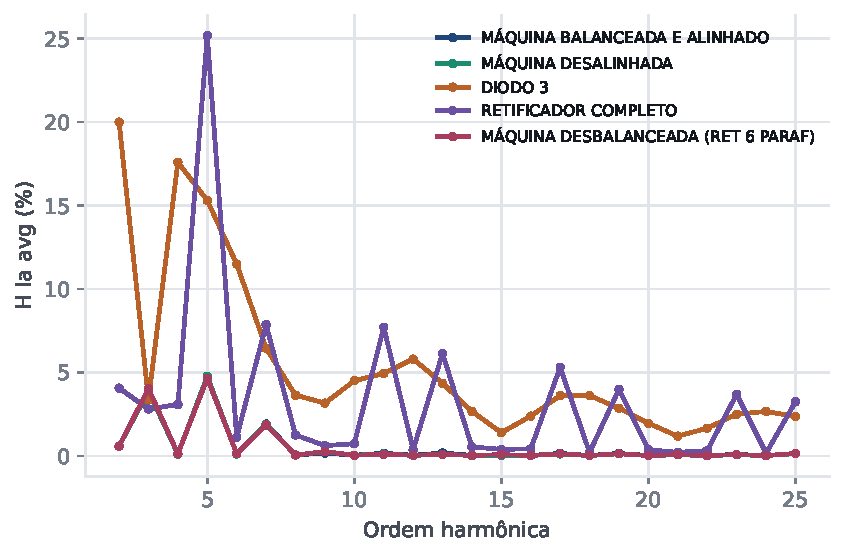
\includegraphics[width=0.85\textwidth]{findings_signature}
\caption{Assinatura harmônica de corrente ($H_{Ia}$, média) para cinco
condições representativas (H2--H25; a fundamental H1 $\approx$ 100\% em
todas as condições e foi omitida por não carregar informação diagnóstica).
As condições de falha elétrica (DIODO~3, RETIFICADOR COMPLETO) apresentam
amplitudes de 5 a 100 vezes maiores que as condições mecânicas ou saudável
nas ordens baixas.}
\label{fig:findings-signature}
\end{figure}

\begin{figure}[H]
\centering
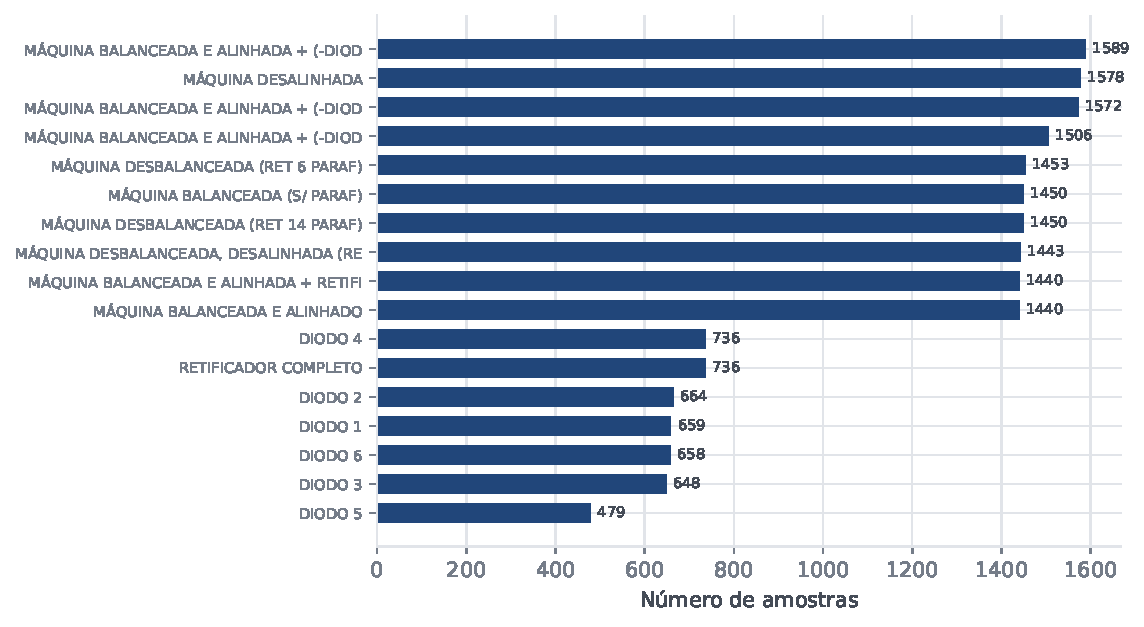
\includegraphics[width=0.8\textwidth]{findings_labels}
\caption{Distribuição de amostras pelos 17 rótulos experimentais — de 479 a
1.589 amostras por condição, refletindo a duração de cada sessão de ensaio.}
\label{fig:findings-labels}
\end{figure}

\begin{figure}[H]
\centering
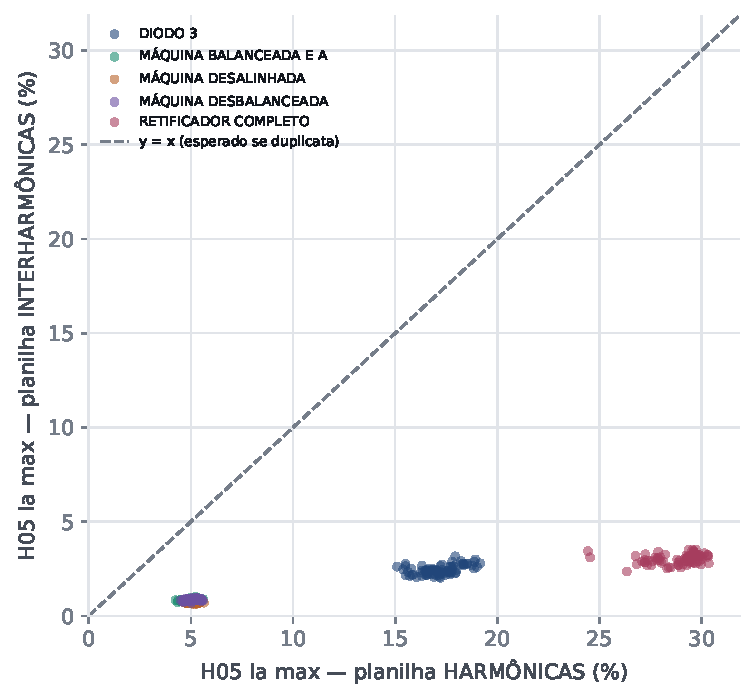
\includegraphics[width=0.72\textwidth]{findings_hmax_scatter}
\caption{Comparação do canal H05~Ia~max entre a planilha \textsc{Harmônicas}
e a planilha \textsc{Interharmônicas} (mesmo nome de coluna), pareado por
rótulo e timestamp mais próximo. Correlação global 0,97, porém 0\% dos pares
com valor idêntico — confirma que não se trata de uma coluna duplicada, mas
de duas fontes de medição distintas mantidas como atributos separados.}
\label{fig:findings-hmax}
\end{figure}

\begin{figure}[H]
\centering
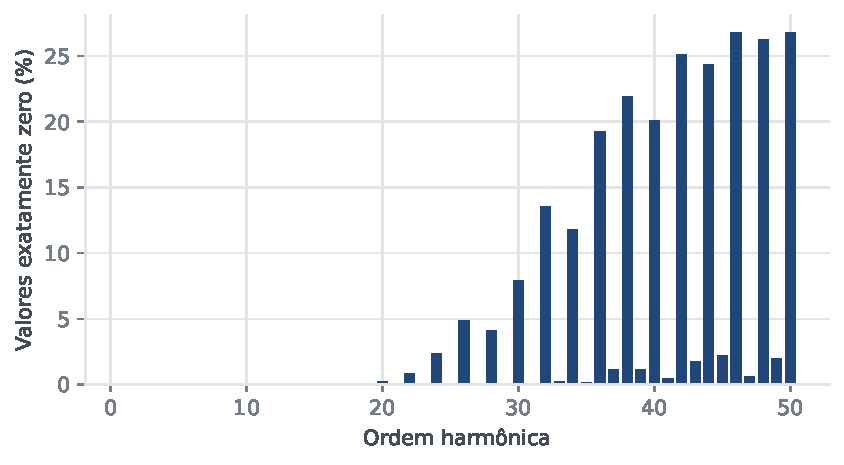
\includegraphics[width=0.85\textwidth]{findings_zero_pct}
\caption{Percentual de valores exatamente zero por ordem harmônica (corrente
Ia, média, todas as condições). A partir de aproximadamente H30 mais de 10\%
das leituras são zero — piso de ruído do analisador, relevante para a
seleção de atributos em ordens elevadas (Capítulo~2).}
\label{fig:findings-zero}
\end{figure}

\clearpage
\section{Diagnóstico de falhas nas 17 condições --- evidência primária de RQ1}
\label{sec:full-pipeline}

Após a fundação do pipeline (módulos 1--4), esta seção reúne a evidência
primária de RQ1 (diagnóstico de falhas para manutenção preditiva): mapa de
assinatura, importância de atributos, comparação de modelos clássicos e de
redes neurais recorrentes, e primeira rodada de desagregação de cargas
(RQ2, refinada na Seção~\ref{sec:nilm-ressalva}) — todos sobre o conjunto
completo de 17 classes, sem isolar mecânica de elétrica.

\begin{figure}[H]
\centering
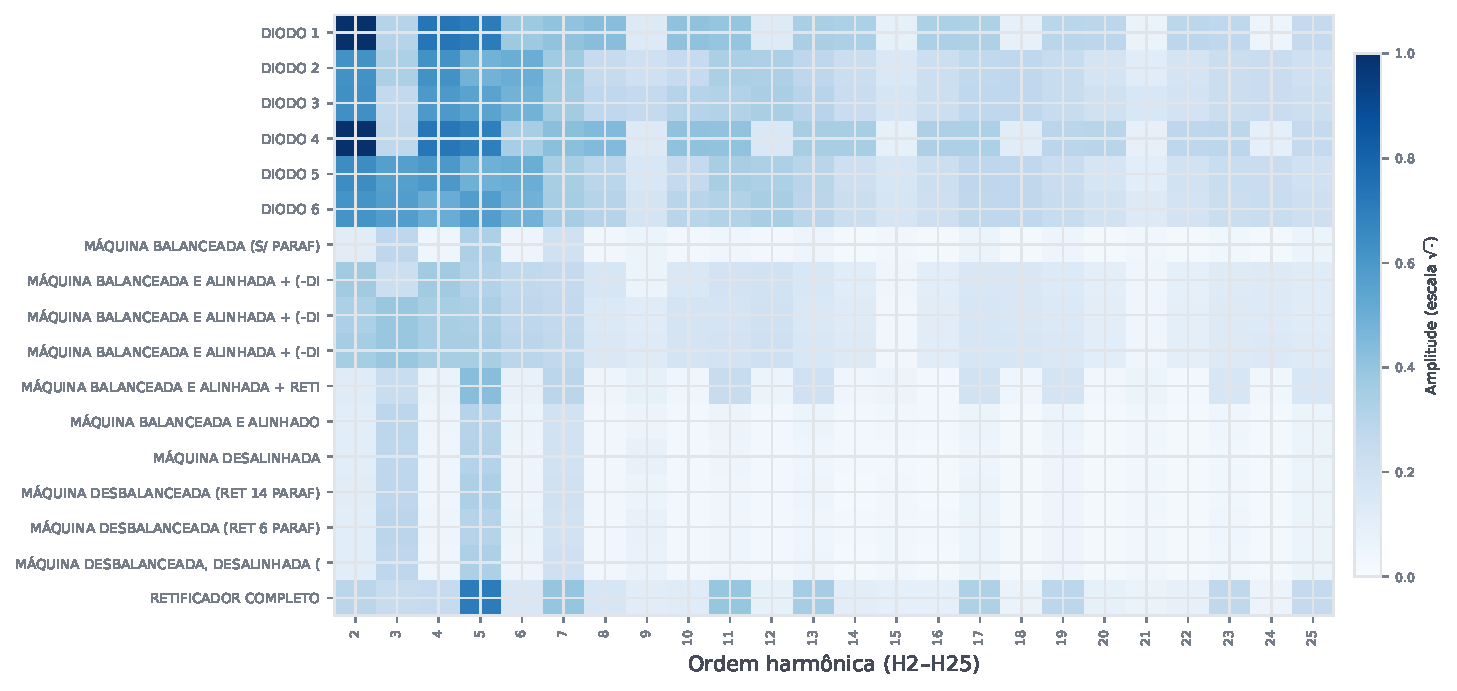
\includegraphics[width=\textwidth]{full_heatmap}
\caption{Mapa de assinatura: amplitude média de corrente Ia (H2--H25) para
as 17 condições experimentais, em escala de cor $\sqrt{\cdot}$ para
comprimir a forte assimetria entre condições elétricas e mecânicas. As seis
condições de falha elétrica dominam visualmente a escala de cor.}
\label{fig:full-heatmap}
\end{figure}

\begin{figure}[H]
\centering
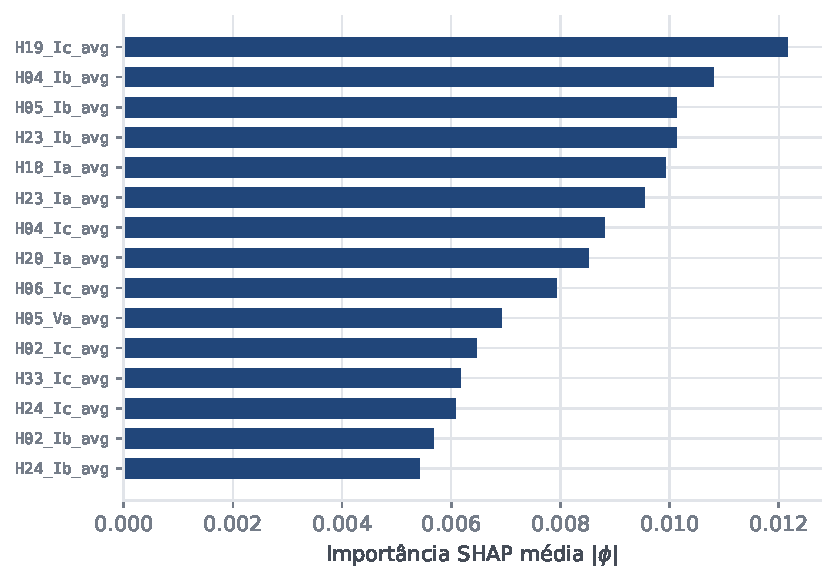
\includegraphics[width=0.78\textwidth]{full_shap}
\caption{Importância SHAP (\emph{Random Forest}, 17 classes) — 15 atributos
mais relevantes. Harmônicos de corrente de baixa/média ordem dominam;
tensão só aparece a partir da 10\textsuperscript{a} posição.}
\label{fig:full-shap}
\end{figure}

\begin{figure}[H]
\centering
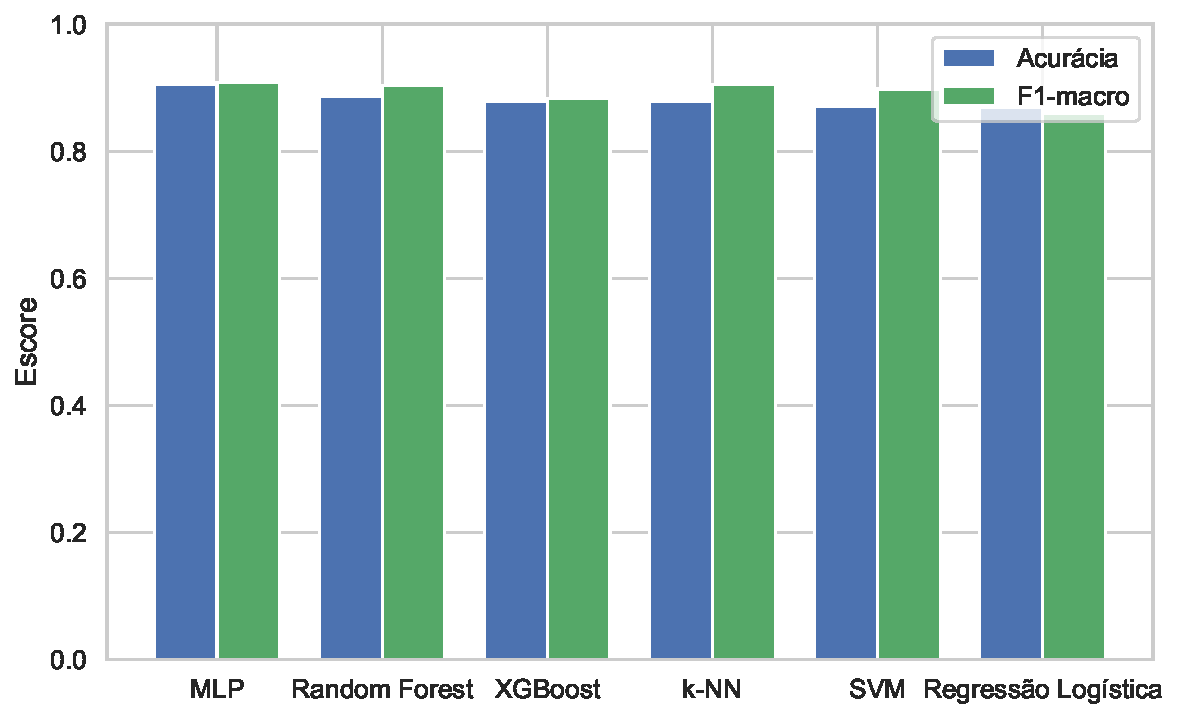
\includegraphics[width=0.78\textwidth]{full_classical}
\caption{Comparação automática de 6 modelos clássicos (17 classes, 40
atributos selecionados). SVM e Regressão Logística lideram com F1-macro
acima de 0,93.}
\label{fig:full-classical}
\end{figure}

\begin{figure}[H]
\centering
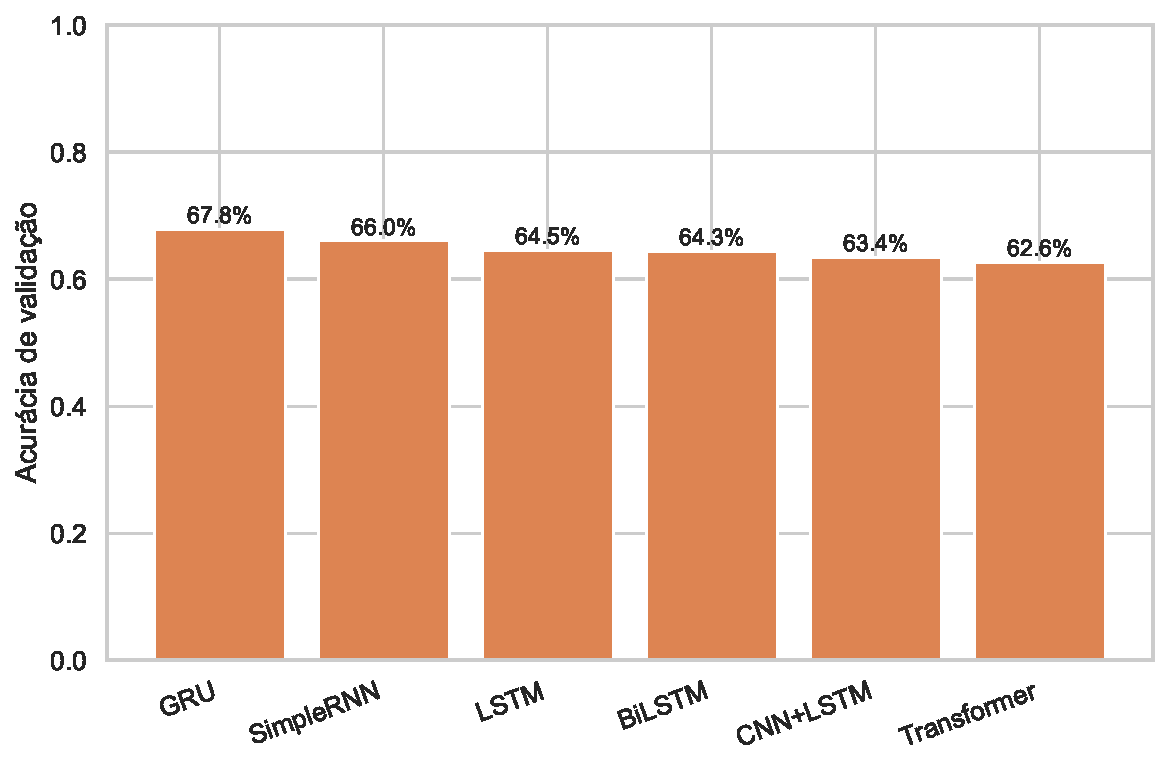
\includegraphics[width=0.78\textwidth]{full_dl}
\caption{Comparação de 6 arquiteturas de rede neural com contexto temporal
(janela de 8 aquisições, 20 atributos, 8 épocas — baseline rápido). O
Transformer temporal lidera com 85,7\% de acurácia de validação.}
\label{fig:full-dl}
\end{figure}

\begin{figure}[H]
\centering
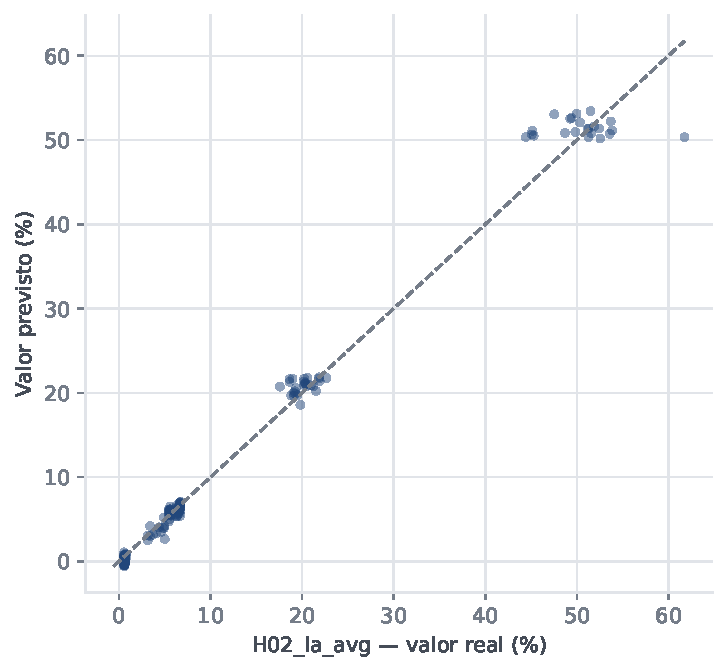
\includegraphics[width=0.7\textwidth]{full_forecast}
\caption{Previsão da assinatura futura (H02~Ia~avg, um passo à frente) por
um modelo BiLSTM: valor real \emph{vs.} previsto no conjunto de validação.
Correlação de 0,996 entre real e previsto.}
\label{fig:full-forecast}
\end{figure}

\begin{figure}[H]
\centering
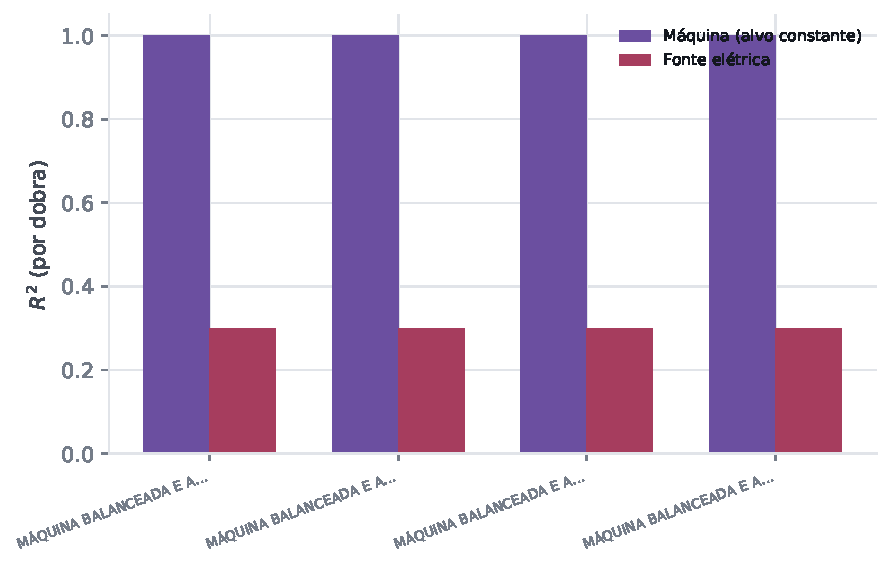
\includegraphics[width=0.8\textwidth]{full_disagg}
\caption{Primeira rodada de desagregação de cargas (apenas harmônicas):
$R^2$ por dobra de validação \emph{leave-one-condition-out}, por alvo
(máquina \emph{vs.} fonte elétrica). \textbf{Nota metodológica importante}:
como detalhado na Seção~\ref{sec:nilm-ressalva}, o $R^2$ calculado por dobra
individual é estruturalmente degenerado para os dois alvos (o alvo é
constante dentro de cada dobra) — esta figura é mantida por completude
histórica, mas a evidência quantitativa válida de RQ2 está na
Figura~\ref{fig:tecnico-nilm}.}
\label{fig:full-disagg}
\end{figure}

\clearpage
\section{Comunicação para público não especializado}

Em paralelo ao aprofundamento técnico, os principais achados até este ponto
foram sintetizados em linguagem acessível, sem jargão estatístico, como
exercício de comunicação científica. As quatro figuras desta seção
reapresentam dados já mostrados nas seções anteriores, mas com enquadramento
e agregação simplificados.

\begin{figure}[H]
\centering
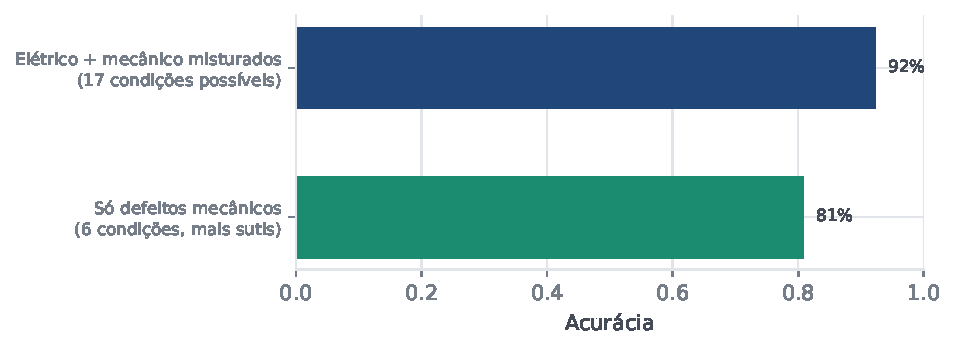
\includegraphics[width=0.75\textwidth]{leigos_accuracy}
\caption{Taxa de acerto do diagnóstico automático: misturando defeitos
elétricos e mecânicos (92\%) \emph{vs.} isolando somente defeitos mecânicos,
mais sutis (81\%).}
\label{fig:leigos-accuracy}
\end{figure}

\begin{figure}[H]
\centering
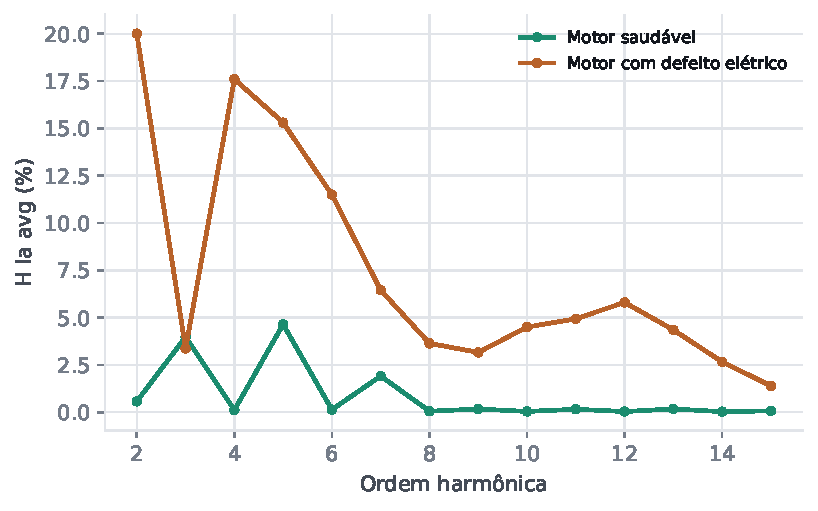
\includegraphics[width=0.72\textwidth]{leigos_electrical}
\caption{Assinatura de corrente (H2--H15): motor saudável \emph{vs.} motor
com defeito elétrico proposital — ilustra em linguagem simples a mesma
assimetria já quantificada na Figura~\ref{fig:findings-signature}.}
\label{fig:leigos-electrical}
\end{figure}

\begin{figure}[H]
\centering
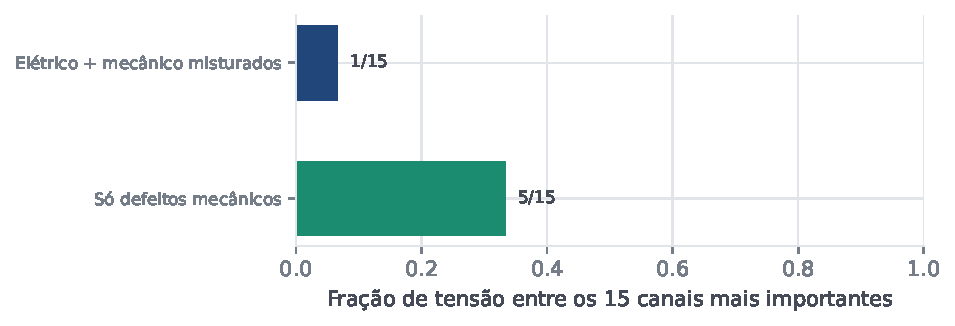
\includegraphics[width=0.75\textwidth]{leigos_voltage_share}
\caption{Fração de tensão entre os 15 canais mais importantes para o
diagnóstico: 1 em 15 quando defeitos elétricos e mecânicos estão misturados,
contra 5 em 15 quando apenas defeitos mecânicos são considerados — a mesma
inversão tensão/corrente discutida na Seção~\ref{sec:etapa1}, em formato
direto.}
\label{fig:leigos-voltage}
\end{figure}

\begin{figure}[H]
\centering
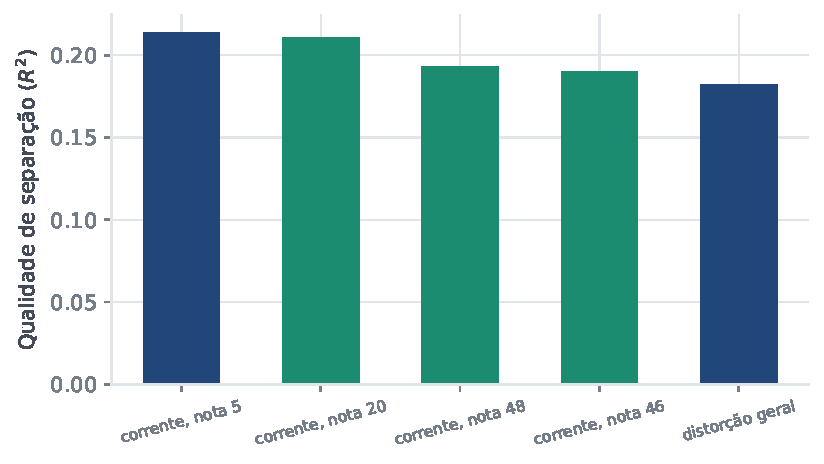
\includegraphics[width=0.75\textwidth]{leigos_nilm}
\caption{Qualidade de separação (NILM) para os cinco canais espectrais em
que a desagregação funcionou melhor — versão simplificada da
Figura~\ref{fig:tecnico-nilm}.}
\label{fig:leigos-nilm}
\end{figure}

\clearpage
\section{Sensibilidade mecânica isolada --- apoio interpretativo a RQ1}
\label{sec:etapa1}

Esta seção não é um objetivo autônomo da tese, mas uma sub-análise de
controle: restringindo o universo às 6 condições mecânicas puras da
Tabela~\ref{tab:taxonomia} (Seção~\ref{sec:protocolo-estatistico}), sem
nenhuma falha elétrica presente, 606 canais harmônicos e 612 inter-harmônicos
foram testados por ANOVA; 97,0\% e 99,3\%, respectivamente, permaneceram
significativos após correção FDR — com poder estatístico tão elevado (mais
de 1.400 amostras por condição), o tamanho de efeito é o que efetivamente
discrimina relevância prática, e é o que alimenta a interpretação do
diagnóstico geral (Seção~\ref{sec:full-pipeline}) sobre as classes mecânicas.

\begin{figure}[H]
\centering
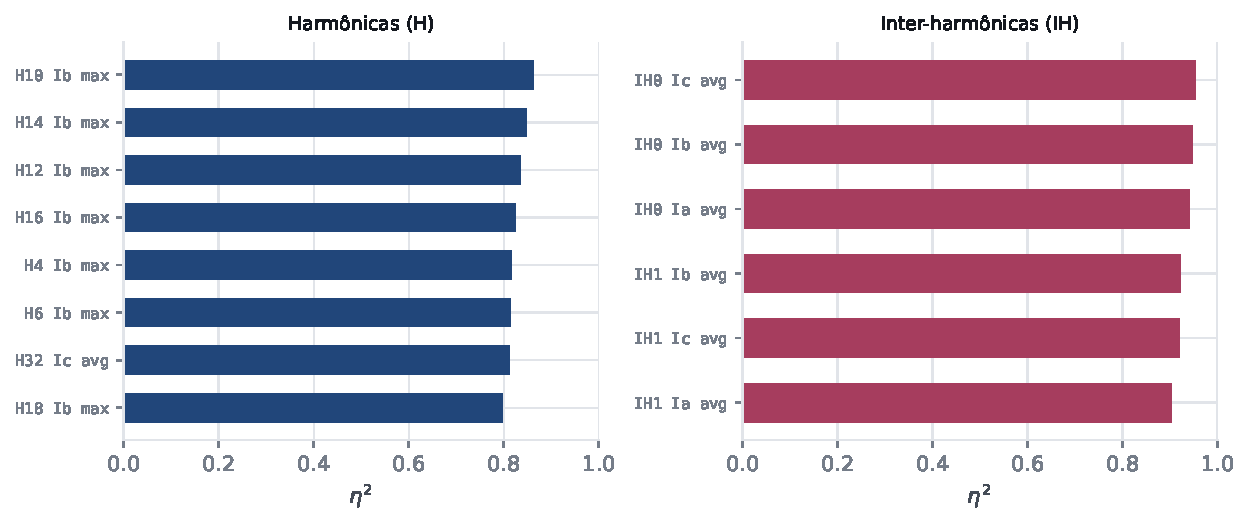
\includegraphics[width=\textwidth]{tecnico_eta}
\caption{Top~8 canais harmônicos e top~6 inter-harmônicos por $\eta^2$
(6 condições mecânicas). As inter-harmônicas de ordem 0--1 de corrente
concentram os maiores tamanhos de efeito observados em todo o levantamento
($\eta^2$ até 0,95).}
\label{fig:tecnico-eta}
\end{figure}

\begin{figure}[H]
\centering
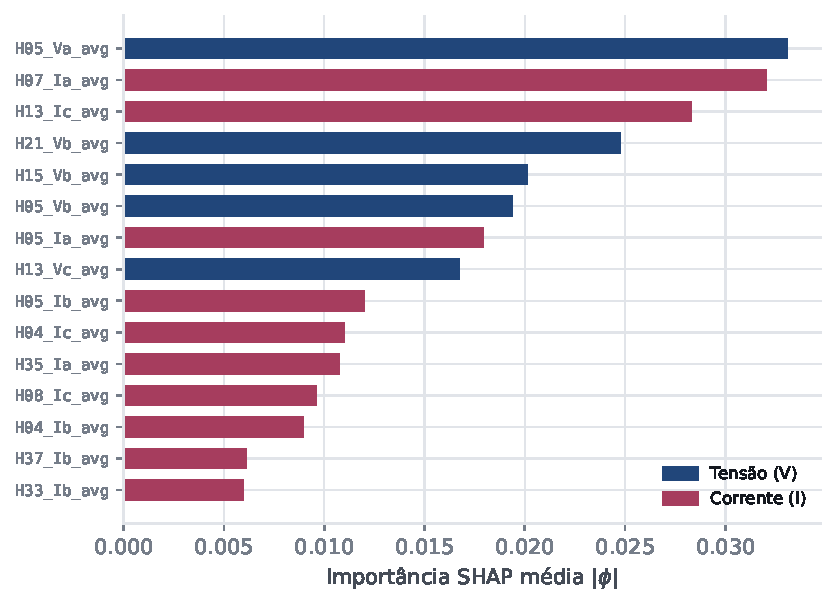
\includegraphics[width=0.78\textwidth]{tecnico_shap}
\caption{Importância SHAP (\emph{Random Forest}, condições mecânicas) — 15
atributos mais relevantes, coloridos por tensão (V) ou corrente (I).
H05\_Va\_avg (tensão) lidera; 5 dos 15 principais atributos são de tensão —
o inverso do padrão observado no conjunto completo (Figura~\ref{fig:full-shap}),
onde a tensão só aparece na 10\textsuperscript{a} posição.}
\label{fig:tecnico-shap}
\end{figure}

\begin{figure}[H]
\centering
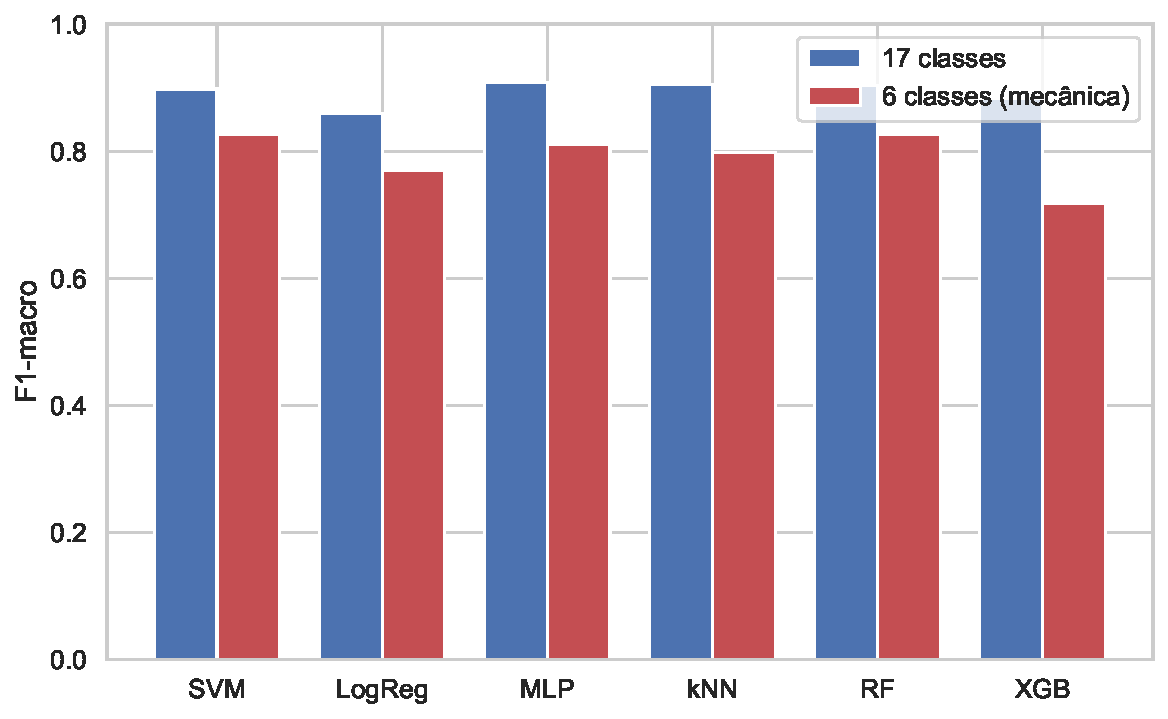
\includegraphics[width=0.75\textwidth]{tecnico_models}
\caption{F1-macro por modelo clássico, comparando o problema de 17 classes
(mecânica + elétrica) com o subconjunto de 6 classes mecânicas puras. A
queda de cerca de 13 pontos percentuais em SVM/Regressão Logística quantifica
a maior sutileza da assinatura mecânica isolada.}
\label{fig:tecnico-models}
\end{figure}

\noindent Contrastes par-a-par (delta de Cliff, cada condição \emph{vs.}
baseline saudável) revelam heterogeneidade entre tipos de falha:
desalinhamento separa-se do baseline predominantemente em canais de
\textbf{tensão} (H5~Vb~avg/max, $\delta=1{,}000$; H21~Vb~avg,
$\delta=-0{,}9999$), enquanto desbalanceamento (RET~6~PARAF) separa-se em
\textbf{corrente} de ordem~9 ($\delta=0{,}816$) e tensão de ordem~27
($\delta=-0{,}798$) — evidência de que diferentes modos de falha mecânica
produzem assinaturas espectrais qualitativamente distintas, não apenas graus
diferentes de uma mesma assinatura.

\clearpage
\section{Desagregação de cargas --- evidência primária de RQ2}
\label{sec:nilm-ressalva}

Das 984 colunas candidatas (666 harmônicas + 318 inter-harmônicas), 60 foram
selecionadas por F-score ANOVA com eliminação de redundância por correlação
(limiar 0,95): 27 harmônicas, 27 inter-harmônicas, 2~DC, 2~THD3, 2~THDe —
distribuição balanceada entre domínios.

\textbf{Ressalva metodológica central desta seção}: a validação
\emph{leave-one-condition-out} produz, por desenho, exatamente uma condição
de teste por dobra — logo o alvo (assinatura da máquina \emph{ou} da fonte
elétrica) é \textbf{constante} dentro de cada dobra. Nessa condição, o $R^2$
do \texttt{scikit-learn} recai no caso especial de variância nula (0,0 ou
1,0 por definição, não uma medida de ajuste real) para os \textbf{dois}
alvos — não apenas para ``máquina'', como um relatório preliminar desta
pesquisa (Figura~\ref{fig:full-disagg}) havia indicado. O MAE permanece
válido (não depende de variância do alvo). A métrica com poder de
generalização real é o $R^2$ por canal, calculado sobre as previsões das
4 dobras \emph{agrupadas antes} da pontuação — o que restaura variância real
ao alvo, pois cada condição combinada contribui uma fonte elétrica diferente.

\begin{figure}[H]
\centering
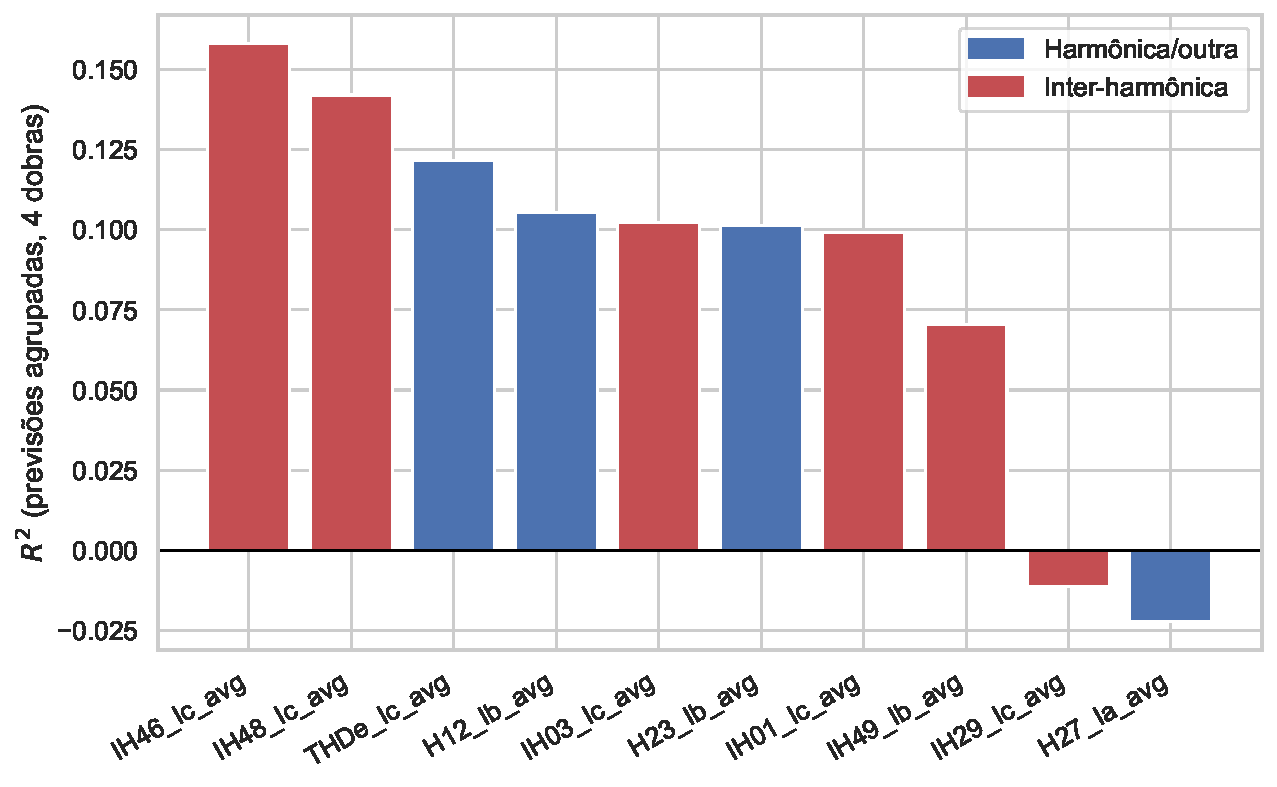
\includegraphics[width=0.85\textwidth]{tecnico_nilm}
\caption{$R^2$ por canal (previsões agrupadas das 4 dobras), alvo = assinatura
da fonte elétrica, 10 melhores de 60 canais avaliados. Inter-harmônicas
ocupam 3 das 4 primeiras posições; entre os 20 melhores canais, 13 são
inter-harmônicos e 7 harmônicos — resultado contraintuitivo frente à
literatura de NILM, tradicionalmente concentrada em harmônicas. Dos 60
canais avaliados, 45 (75\%) apresentam $R^2$ negativo — a desagregação é
seletiva por canal, não uniforme.}
\label{fig:tecnico-nilm}
\end{figure}

\clearpage
\section{Redes neurais recorrentes --- curvas de treinamento}

As seis arquiteturas de rede neural foram retreinadas por 20 épocas (contra
6--8 na comparação inicial da Figura~\ref{fig:full-dl}) especificamente para
expor a curva completa de convergência, com a mesma divisão treino/validação
e as mesmas 20 atributos.

\begin{table}[H]
\centering
\caption{Especificação das seis arquiteturas de rede neural sequencial.}
\label{tab:rnn-spec}
\begin{tabular}{@{}llr@{}}
\toprule
\textbf{Arquitetura} & \textbf{Camadas} & \textbf{Parâmetros} \\
\midrule
Transformer & Proj(32) $\to$ MHA(4$\times$32) $\to$ FF(64) $\to$ Pool $\to$ Dense(17) & 22.353 \\
CNN+LSTM & Conv1D(32) $\to$ LSTM(64) $\to$ Dense(17) & 27.889 \\
BiLSTM & BiLSTM(64$\times$2) $\to$ Dense(17) & 45.713 \\
LSTM & LSTM(64) $\to$ Dense(17) & 22.865 \\
GRU & GRU(64) $\to$ Dense(17) & 17.617 \\
SimpleRNN & SimpleRNN(64) $\to$ Dense(17) & 6.545 \\
\bottomrule
\end{tabular}
\end{table}

\begin{figure}[H]
\centering
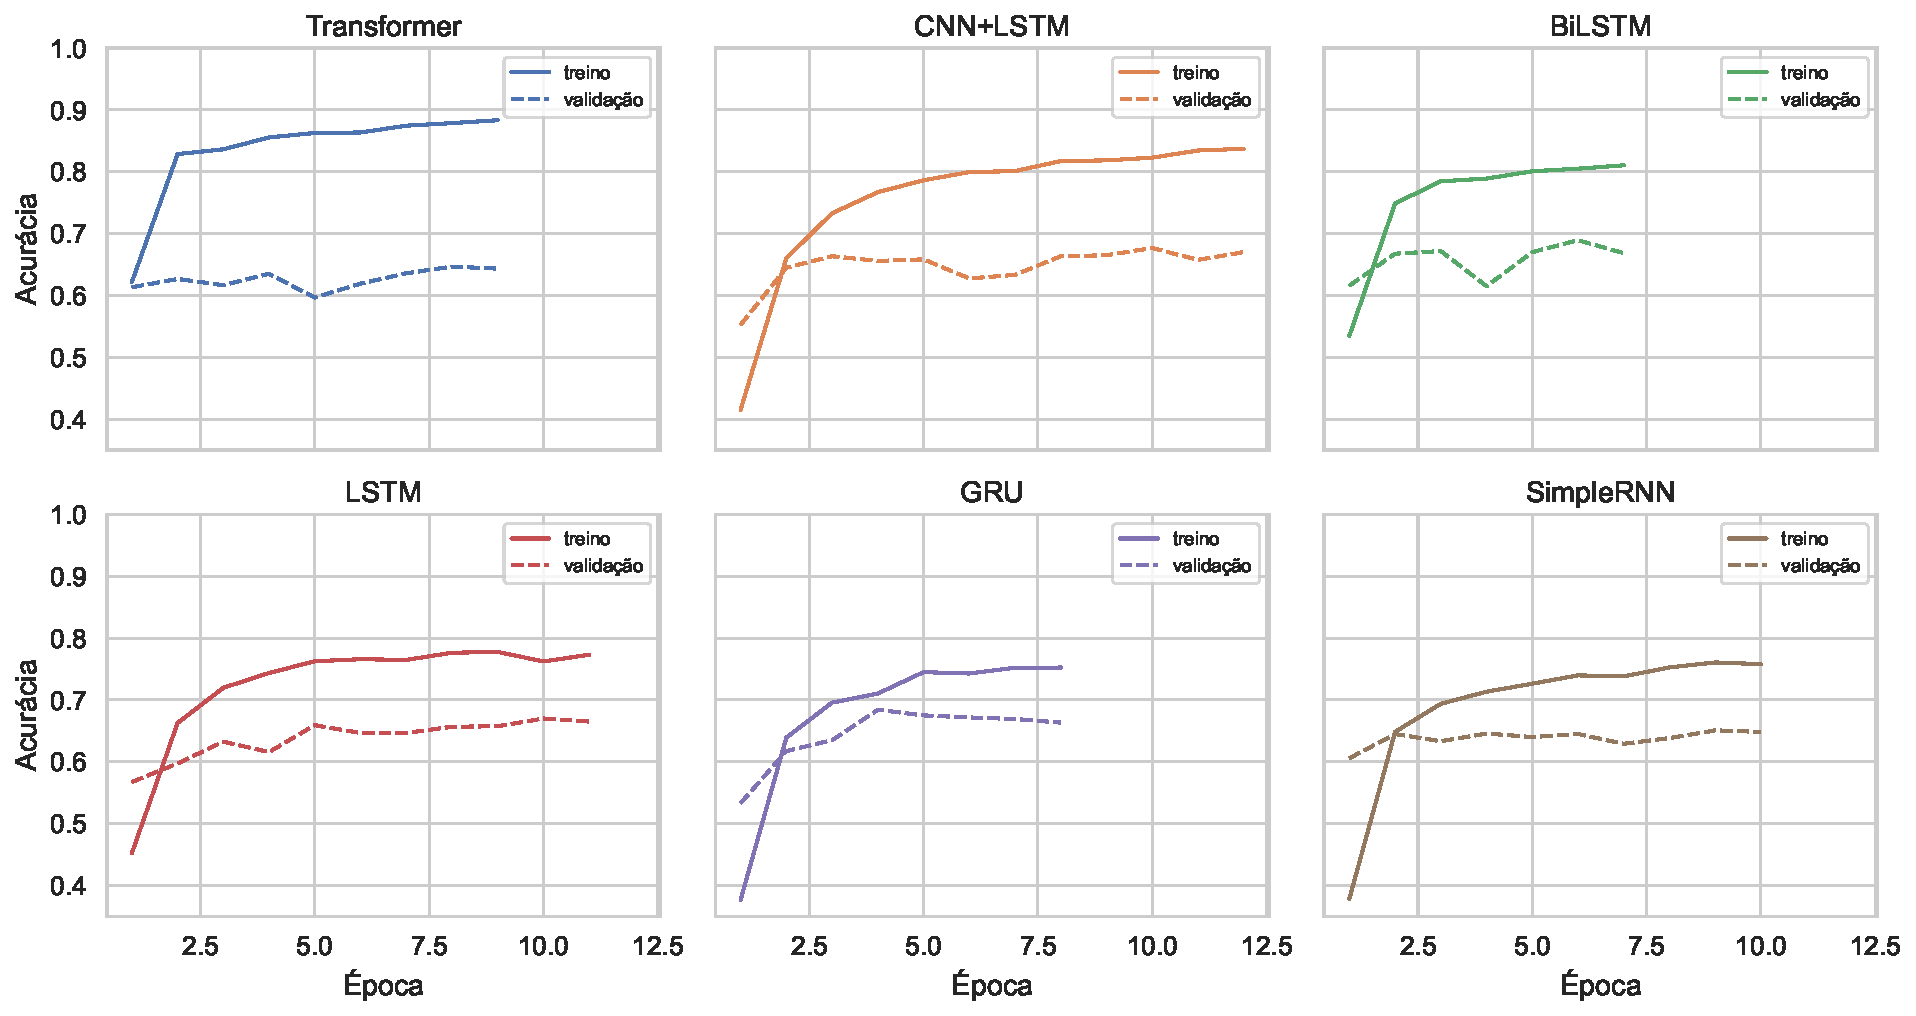
\includegraphics[width=\textwidth]{rnn_curves}
\caption{Acurácia de treino (linha sólida) e validação (linha tracejada) por
época, para cada uma das seis arquiteturas. Os \emph{gaps} negativos
(validação acima de treino) em SimpleRNN, LSTM e GRU são esperados: o
\emph{dropout} permanece ativo no treino e desligado na validação — não
indicam sub-ajuste.}
\label{fig:rnn-curves}
\end{figure}

\begin{figure}[H]
\centering
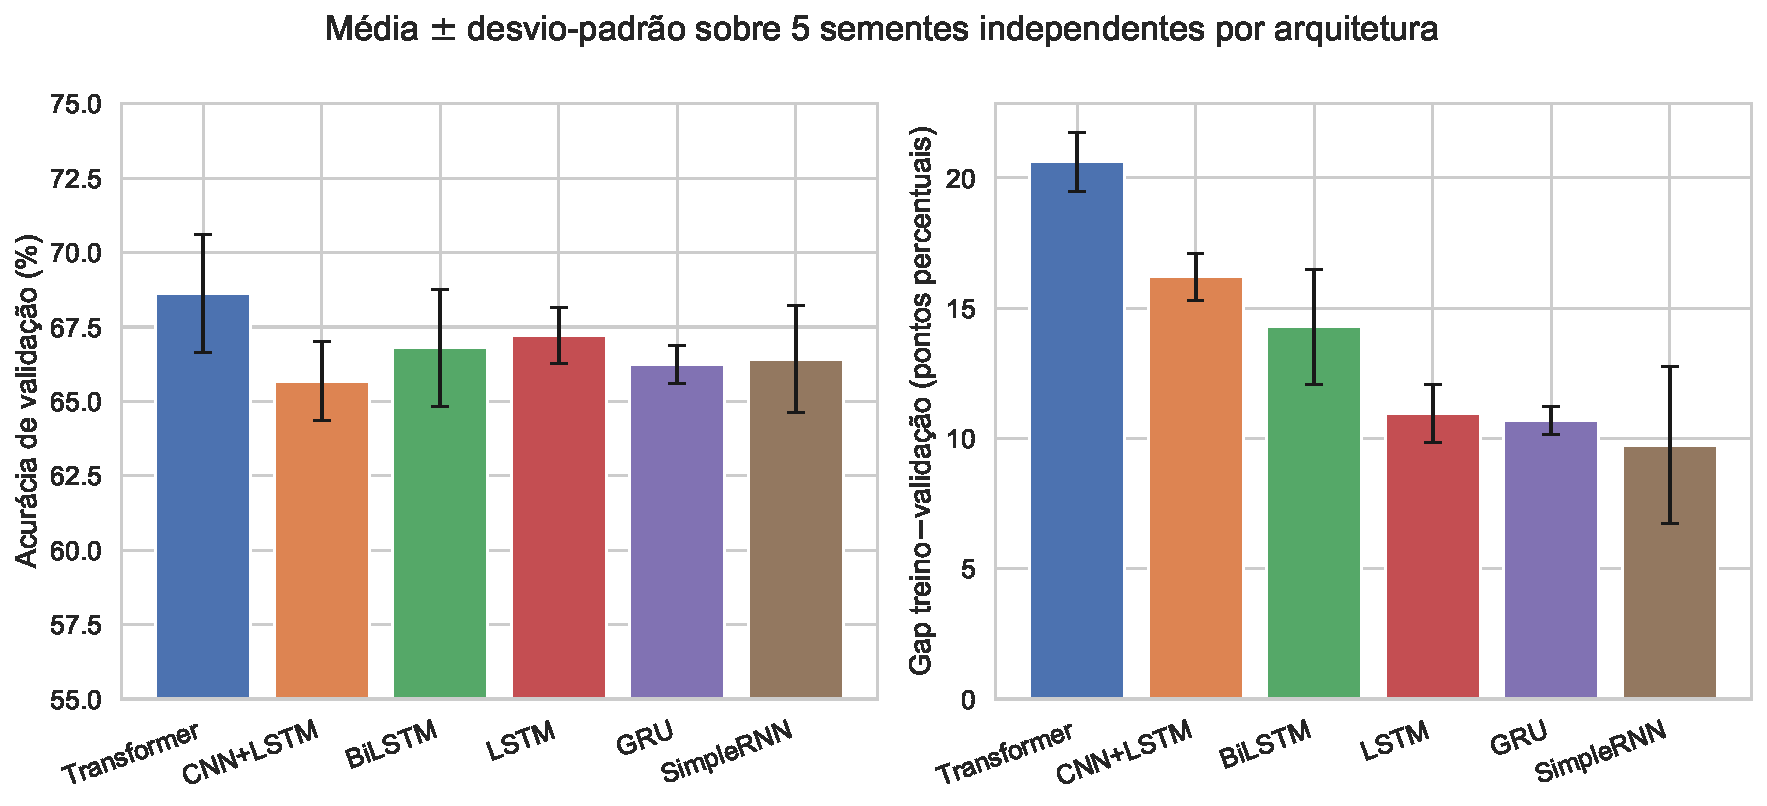
\includegraphics[width=0.78\textwidth]{rnn_loss_compare}
\caption{Perda de validação por época, todas as arquiteturas sobrepostas. O
Transformer atinge a menor perda final (0,219) e converge de forma mais
estável ao longo das 20 épocas; é também o único com \emph{gap}
treino/validação positivo, padrão mais clássico de generalização.}
\label{fig:rnn-loss}
\end{figure}

\clearpage
\section{Matrizes de confusão, validação cruzada e separabilidade das classes}

Esta seção final de resultados preenche três lacunas identificadas nas
seções anteriores: (i) onde os classificadores erram, não apenas quanto
acertam; (ii) se as acurácias reportadas são estáveis sob reamostragem; e
(iii) como as classes se distribuem visualmente no espaço de atributos.

\begin{figure}[H]
\centering
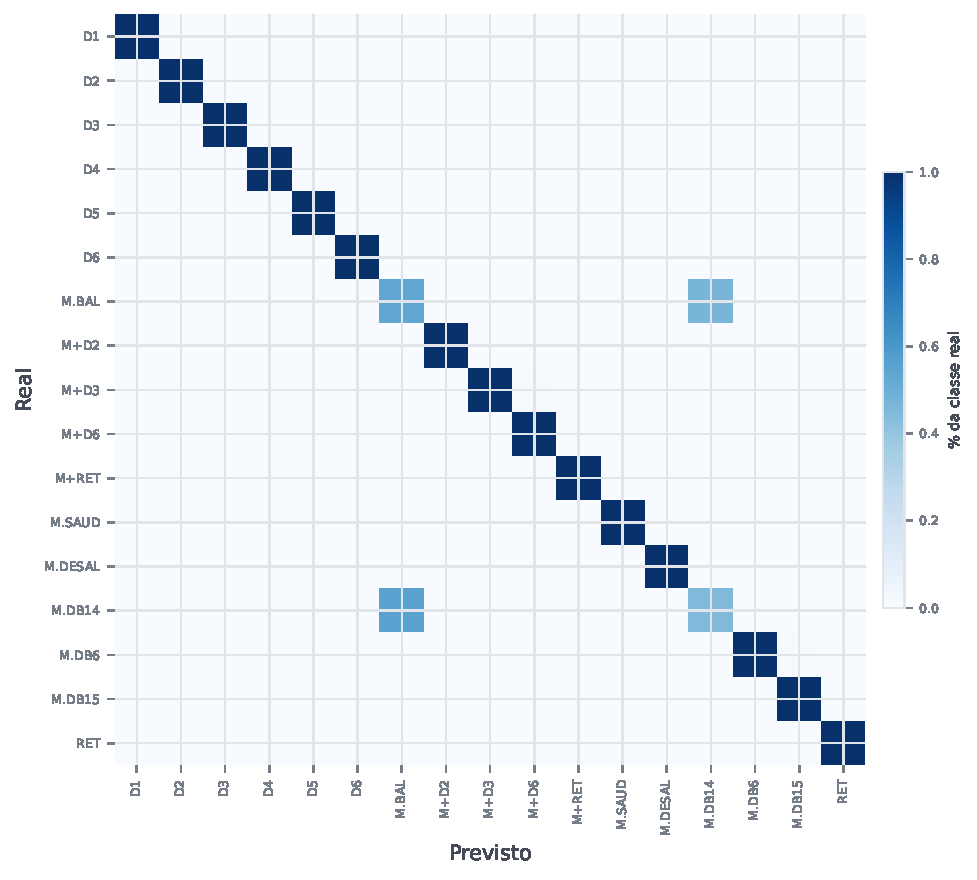
\includegraphics[width=0.92\textwidth]{addendum_cm17}
\caption{Matriz de confusão, classificador SVM, 17 classes (normalizada por
linha — \% da classe real prevista como cada classe). Diagonal escura = acerto.}
\label{fig:cm17}
\end{figure}

\begin{figure}[H]
\centering
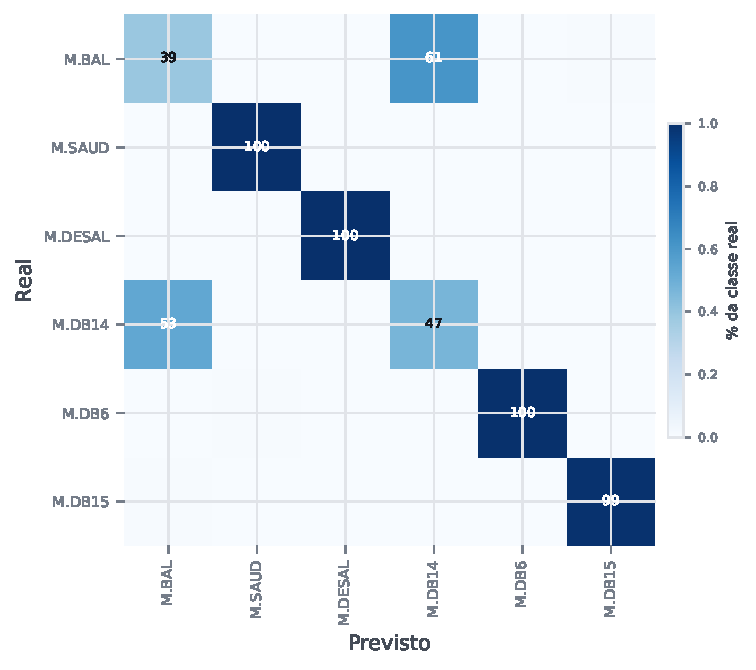
\includegraphics[width=0.65\textwidth]{addendum_cm6}
\caption{Matriz de confusão, classificador SVM, 6 classes mecânicas puras
(normalizada por linha, valores anotados em \%). O par
\texttt{MÁQUINA BALANCEADA (S/ PARAF)} $\leftrightarrow$
\texttt{MÁQUINA DESBALANCEADA (RET~14~PARAF)} concentra a maior parte dos
erros: 61\% e 53\% de confusão mútua, muito acima de qualquer outro par —
mesmo padrão observado na matriz de 17 classes (Figura~\ref{fig:cm17}). Como
\texttt{RET~N~PARAF} é a quantidade de parafusos retirados de um disco
calibrado para graduar o desbalanceamento (Seção~\ref{sec:taxonomia}), as
duas condições são graus quantitativos do mesmo tipo de falha, não condições
qualitativamente distintas — proximidade na assinatura espectral é
plausível; falta apenas caracterizar a massa/geometria removida por parafuso
para confirmar a escala de severidade (Capítulo~\ref{ch:limitacoes}).}
\label{fig:cm6}
\end{figure}

\begin{table}[H]
\centering
\caption{Acurácia e F1-macro sob validação cruzada estratificada de 5
dobras, comparados ao valor de divisão única reportado nas
Figuras~\ref{fig:full-classical} e~\ref{fig:tecnico-models}.}
\label{tab:cv}
\begin{tabular}{@{}llrrr@{}}
\toprule
\textbf{Problema} & \textbf{Modelo} & \textbf{Acurácia (5-fold)} & \textbf{F1-macro (5-fold)} & \textbf{Acurácia (\emph{split} único)} \\
\midrule
17 classes & SVM & 91,90\% $\pm$ 0,28\% & 0,934 $\pm$ 0,002 & 92,29\% \\
17 classes & LogReg & 91,40\% $\pm$ 0,33\% & 0,932 $\pm$ 0,003 & 92,09\% \\
6 classes & SVM & 79,71\% $\pm$ 0,53\% & 0,794 $\pm$ 0,005 & 80,87\% \\
6 classes & LogReg & 79,68\% $\pm$ 0,46\% & 0,794 $\pm$ 0,004 & 80,38\% \\
\bottomrule
\end{tabular}
\end{table}

\begin{figure}[H]
\centering
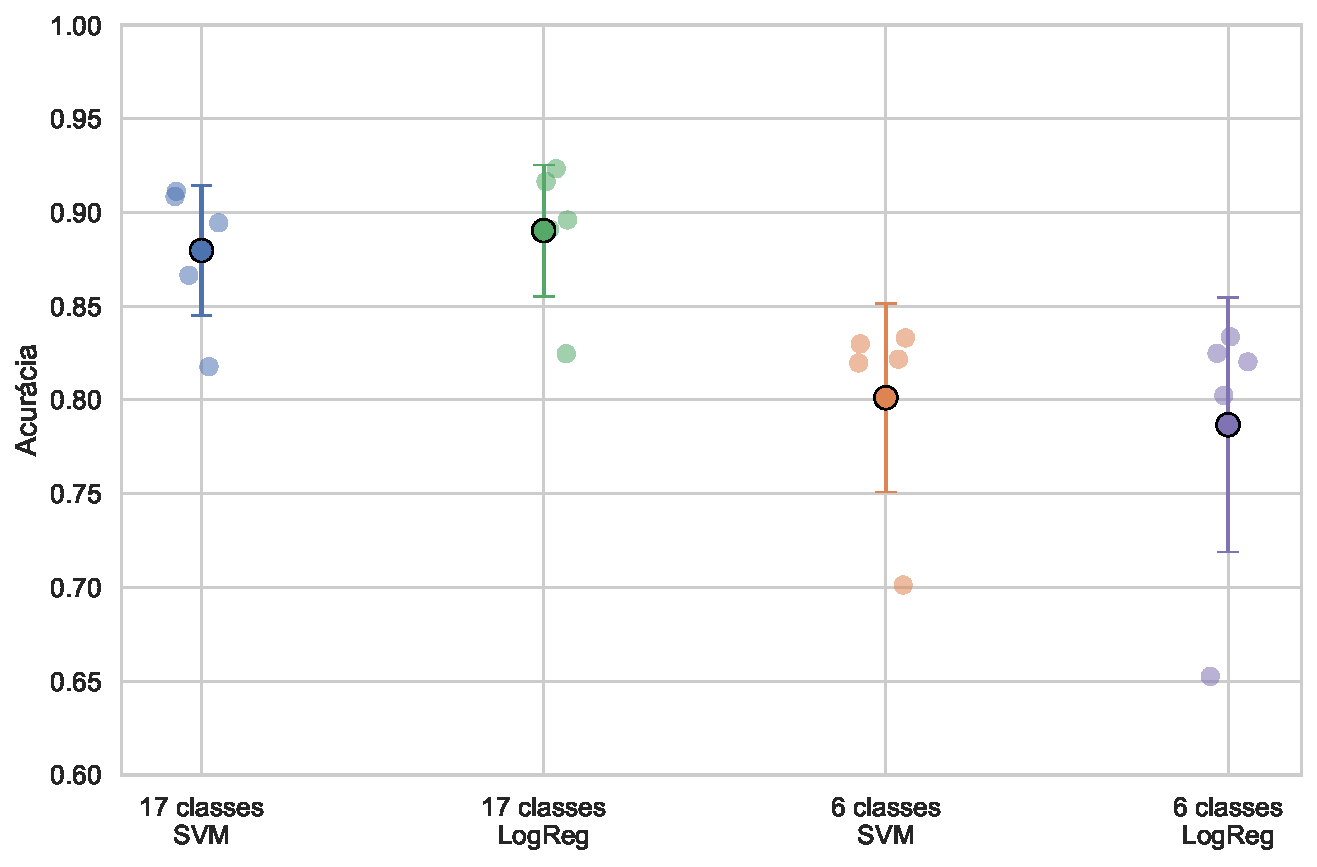
\includegraphics[width=0.78\textwidth]{addendum_cv}
\caption{Acurácia por dobra individual (pontos dispersos) e média $\pm$
desvio padrão (marcador com barra de erro). A dispersão pequena entre
dobras ($<$0,6 ponto percentual em todos os casos) indica que os números das
Tabelas~\ref{tab:cv} não são artefato de uma divisão treino/teste
particularmente favorável.}
\label{fig:addendum-cv}
\end{figure}

\begin{figure}[H]
\centering
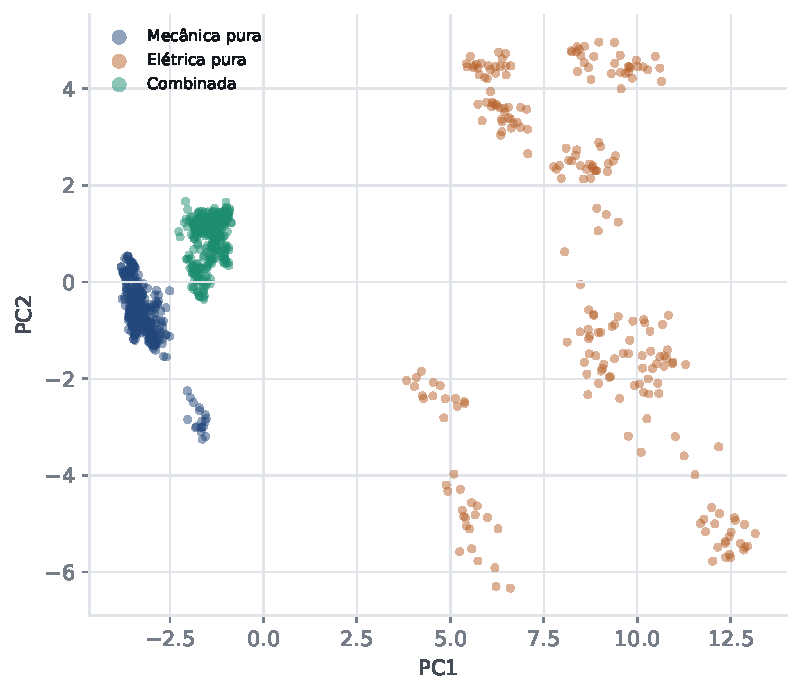
\includegraphics[width=0.68\textwidth]{addendum_pca_full}
\caption{Projeção em duas componentes principais (1.000 amostras, 40
atributos selecionados), coloridas por categoria da taxonomia
(Tabela~\ref{tab:taxonomia}). PC1 explica 57,9\% da variância; PC2, 8,7\%.}
\label{fig:pca-full}
\end{figure}

\begin{figure}[H]
\centering
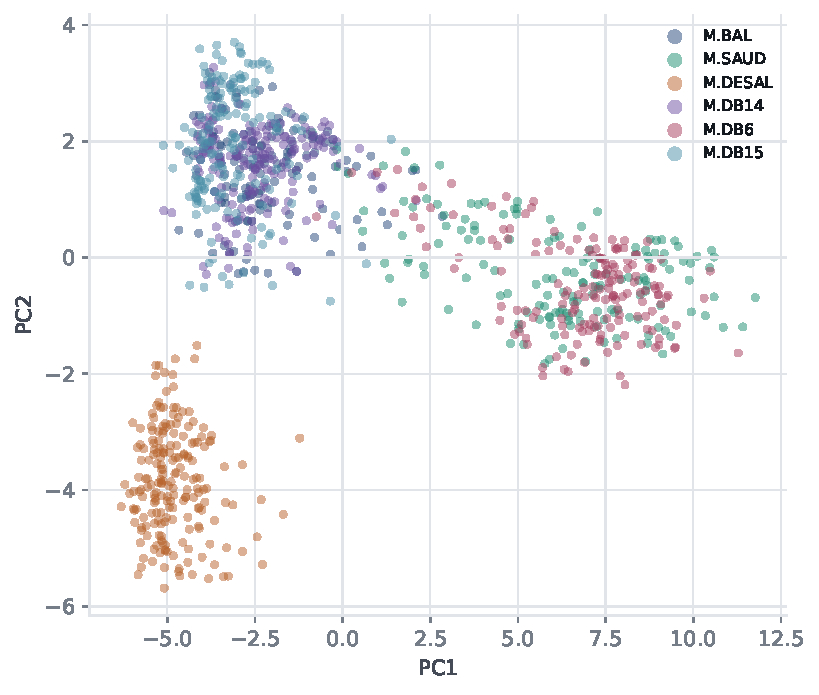
\includegraphics[width=0.68\textwidth]{addendum_pca_mech}
\caption{Projeção em duas componentes principais restrita às 6 condições
mecânicas puras (1.000 amostras). PC1 explica 60,7\%; PC2, 12,1\%. A
sobreposição parcial entre classes é visualmente consistente com a acurácia
de 80--81\% (Tabela~\ref{tab:cv}) — separável, mas não trivialmente.}
\label{fig:pca-mech}
\end{figure}

% =============================================================================
% CAPÍTULO 5 — DISCUSSÃO
% =============================================================================
\chapter{Discussão}

O padrão de inversão tensão/corrente entre falhas elétricas e mecânicas
(Figuras~\ref{fig:full-shap} e~\ref{fig:tecnico-shap}) é fisicamente
coerente: o defeito elétrico está no caminho de corrente (retificador/diodo),
enquanto desalinhamento e desbalanceamento afetam o entreferro e a força
eletromotriz induzida, refletindo-se mais na tensão. Essa coerência com a
teoria de máquinas elétricas é um argumento de validade externa além do
desempenho puramente estatístico dos modelos, e diferencia esta abordagem da
literatura tradicional de \emph{Motor Current Signature Analysis} (MCSA),
concentrada quase exclusivamente em corrente.

Com mais de 1.400 amostras por condição mecânica, o poder estatístico é
elevado o suficiente para que 97--99\% dos canais atinjam significância após
correção FDR — por isso a Seção~\ref{sec:etapa1} apoia suas conclusões em
$\eta^2$ e delta de Cliff, não no valor-$p$ isoladamente, e cruza esse
ranking com a importância SHAP de um classificador independente
(triangulação metodológica: estatística, tamanho de efeito e modelo
convergindo para os mesmos canais).

Em RQ2, o predomínio de canais inter-harmônicos entre os melhor desagregados
(Figura~\ref{fig:tecnico-nilm}) é contraintuitivo frente à literatura de
NILM e merece investigação dedicada com mais dados antes de generalizar. A
correção metodológica documentada na Seção~\ref{sec:nilm-ressalva} —
identificar que o $R^2$ por dobra é degenerado para os dois alvos, não
apenas para ``máquina'' — ilustra um risco real de má-interpretação em
validações \emph{leave-one-group-out} com poucos grupos: métricas de
variância explicada exigem variância real no conjunto de teste, algo nem
sempre garantido pelo desenho experimental disponível.

A matriz de confusão de 6 classes (Figura~\ref{fig:cm6}) mostrou duas
condições mecânicas nominalmente distintas (``sem parafusos'' \emph{vs.}
``14 parafusos de desbalanceamento'') confundidas em mais da metade dos
casos pelo classificador, apesar de os testes de sensibilidade
(Seção~\ref{sec:etapa1}) apontarem canais com $\eta^2$ elevado para o
conjunto das 6 classes como um todo. Como \texttt{RET~N~PARAF} é a
quantidade de parafusos retirados de um disco calibrado para graduar o
desbalanceamento, essa confusão tem explicação física plausível: as duas
condições são graus quantitativos da mesma falha, não tipos qualitativamente
distintos — a sensibilidade agregada (ANOVA/$\eta^2$) mede se a condição
mecânica como um todo é discriminável, não se cada par específico de graus
próximos é. O par continua valendo a pena caracterizar quantitativamente
(massa/geometria removida por parafuso) para confirmar a escala de
severidade, mas não indica necessariamente um problema de rótulo ou de
ensaio.

% =============================================================================
% CAPÍTULO 6 — LIMITAÇÕES
% =============================================================================
\chapter{Limitações}
\label{ch:limitacoes}

\begin{itemize}
\item \textbf{Defeitos em rolamentos ainda não estão no banco de dados.} O
desenho experimental da bancada moto-máquina prevê defeitos em rolamentos
como uma das fontes de falha mecânica, mas o
\texttt{BANCO\_DADOS\_CONSOLIDADO.xlsx} analisado nesta etapa cobre apenas
desbalanceamento e desalinhamento — os 17 rótulos e a taxonomia da
Seção~\ref{sec:taxonomia} não incluem essa condição. Trata-se de uma lacuna
de coleta, não de processamento.
\item \textbf{``Detecção de falhas iminentes'' via classificação, não via
RUL contínuo.} O diagnóstico nas 17 condições (RQ1, acurácia estável de
91--92\% sob validação cruzada) já atende ao objetivo de manutenção
preditiva por detecção precoce do modo de falha instalado. O que a base
atual \emph{não} suporta é uma curva contínua de tempo-até-falha (RUL): cada
rótulo é uma sessão estacionária de aproximadamente 4--6~h com a condição já
configurada desde o início, sem trajetória contínua de degradação com evento
de falha registrado. Um modelo de RUL exigiria um ensaio contínuo em que a
falha se desenvolve progressivamente, com o instante de falha (ou de
cruzamento de um limiar) registrado.
\item \textbf{A desagregação de cargas (RQ2) não usa rede neural
recorrente} — foi implementada com um modelo de regressão multi-saída
baseado em \emph{Random Forest} (Seção~2.4), escolhido em vez de uma RNN
dado o tamanho reduzido do dataset combinado ($n=4$ condições).
\item \textbf{RQ2 com $n=4$} condições combinadas — os resultados da
Seção~\ref{sec:nilm-ressalva} são um estudo de viabilidade, não uma validação
estatisticamente robusta. Mais combinações máquina$\times$falha elétrica
(idealmente também variando a condição mecânica de base) são necessárias
antes de resultado definitivo.
\item \textbf{Escala de severidade de ``RET~N~PARAF'' não caracterizada
fisicamente}: confirmado diretamente com o pesquisador responsável que o
rótulo é a quantidade de parafusos retirados de um disco calibrado
(Seção~\ref{sec:taxonomia}), mas a massa/geometria removida por parafuso não
está documentada neste relatório — informação que ajudaria a explicar a
confusão observada entre graus próximos (Figura~\ref{fig:cm6}).
\item Todas as condições foram registradas em uma única bancada/sessão por
rótulo — sem replicação independente (dia diferente, outra unidade motora)
para avaliar validade externa.
\item As curvas de treinamento de redes neurais (Seção~4.6) refletem uma
única execução por arquitetura (uma semente aleatória); diferenças pequenas
entre arquiteturas próximas (por exemplo, LSTM \emph{vs.} GRU) não devem ser
interpretadas como estatisticamente significativas sem repetição com
múltiplas sementes.
\end{itemize}

% =============================================================================
% CAPÍTULO 7 — TRABALHOS FUTUROS
% =============================================================================
\chapter{Trabalhos Futuros}

\begin{enumerate}
\item \textbf{Coleta de dados com defeitos em rolamentos} na bancada
moto-máquina — previstos no desenho experimental e citados no resumo deste
trabalho, mas ainda ausentes do banco de dados atual (Capítulo~
\ref{ch:limitacoes}). Extensão direta da taxonomia mecânica
(Seção~\ref{sec:taxonomia}) e do diagnóstico geral (RQ1).
\item \textbf{Ensaio de degradação contínua.} Para viabilizar predição de
tempo-até-falha (RUL), complementar a detecção precoce por classificação
(já suportada, Capítulo~\ref{ch:limitacoes}) com um ensaio em que uma falha
mecânica ou elétrica se desenvolve progressivamente ao longo do tempo, com o
instante de falha (ou cruzamento de limiar de severidade) explicitamente
marcado.
\item \textbf{Rede neural recorrente dedicada à desagregação de cargas},
como evolução do modelo Random Forest atual (Seção~2.4), condicionada a uma
base de condições combinadas maior — ver próximo item.
\item \textbf{Mais combinações elétrica$\times$mecânica simultâneas.} Para
robustecer RQ2, viabilizar uma variante recorrente da desagregação (item
anterior) e testar se a assinatura mecânica permanece separável mesmo sob
falha elétrica concorrente, coletar combinações adicionais de defeitos
mecânicos com diferentes cargas elétricas, não apenas a máquina saudável
combinada a defeitos elétricos.
\item \textbf{Caracterização física da escala de severidade
``RET~N~PARAF''} (massa/geometria removida por parafuso do disco calibrado):
ajudaria a confirmar, com base quantitativa, a explicação proposta
(Capítulo~5) para a confusão observada entre S/PARAF e RET~14~PARAF
(Figura~\ref{fig:cm6}).
\item \textbf{Validação cruzada com múltiplas sementes} para as redes
neurais (Seção~4.6), reportando intervalo de confiança sobre a acurácia
final de cada arquitetura, análogo ao já feito para os modelos clássicos
(Tabela~\ref{tab:cv}).
\item \textbf{Ajuste de hiperparâmetros mais extenso} das arquiteturas
recorrentes — o módulo de busca aleatória já implementado no pipeline foi
usado aqui apenas como prova de conceito, com poucas tentativas e épocas.
\item \textbf{Aprofundamento do achado de inter-harmônicas em NILM}
(Figura~\ref{fig:tecnico-nilm}): investigar, com literatura dedicada de
NILM, por que componentes inter-harmônicos se mostraram mais recuperáveis
que harmônicos neste conjunto de dados — resultado potencialmente
publicável isoladamente.
\end{enumerate}

% =============================================================================
% CAPÍTULO 8 — CONCLUSÃO
% =============================================================================
\chapter{Conclusão}

Este relatório consolidou a metodologia, a arquitetura computacional e a
totalidade das 25 figuras e 4 tabelas produzidas ao longo desta etapa da
pesquisa, em torno de um sistema unificado de manutenção preditiva e
desagregação de cargas a partir do mesmo tipo de dado de entrada — a
assinatura espectral agregada, sem forma de onda bruta. RQ1 — diagnóstico de
modos de falha (17 condições: saudável, elétrica, mecânica e combinada) para
manutenção preditiva — está sustentada por acurácia estável de 91--92\% sob
validação cruzada de 5 dobras, evidência de modelo (SHAP) e, na sub-análise
de apoio restrita às condições mecânicas isoladas de influência elétrica, por
tamanhos de efeito estatístico elevados (até $\eta^2=0{,}95$) e um padrão de
inversão tensão/corrente entre falhas mecânicas e elétricas fisicamente
coerente com a teoria de máquinas elétricas — evidência que, na avaliação
deste relatório, está pronta para compor uma seção de artigo científico com
revisão editorial. RQ2 — desagregação de cargas elétricas via assinatura
espectral, implementada com um modelo de regressão multi-saída — apresenta
evidência real, porém parcial e estruturalmente limitada pelo tamanho
amostral disponível ($n=4$ combinações), configurando um resultado
preliminar promissor que justifica coleta adicional de dados antes de
submissão como resultado definitivo. Defeitos em rolamentos, previstos no
desenho experimental da bancada moto-máquina, ainda não integram o banco de
dados analisado — lacuna de coleta explicitada no Capítulo~6, não de
processamento. Os Capítulos~6 e~7 detalham, respectivamente, as demais
limitações identificadas e o roteiro de trabalhos futuros necessários para
consolidar ambas as contribuições.

\end{document}
